%% Submissions for peer-review must enable line-numbering
%% using the lineno option in the \documentclass command.
%%
%% Preprints and camera-ready submissions do not need
%% line numbers, and should have this option removed.
%%
%% Please note that the line numbering option requires
%% version 1.1 or newer of the wlpeerj.cls file, and
%% the corresponding author info requires v1.2

\documentclass[fleqn,10pt,lineno]{wlpeerj} % for journal submissions

% ZNK -- Adding headers for pandoc

\setlength{\emergencystretch}{3em}
\providecommand{\tightlist}{
\setlength{\itemsep}{0pt}\setlength{\parskip}{0pt}}
\usepackage{lipsum}
\usepackage[unicode=true]{hyperref}
\usepackage{longtable}



\usepackage{lipsum} \usepackage{textcomp, rotating}

\title{Detecting the impact of land cover change on observed rainfall.}

\author[1]{Chun X. Liang}

\author[1]{Floris F. van Ogtrop}

\author[1]{R. Willem Vervoort}

\corrauthor[1]{R. Willem Vervoort}{\href{mailto:willem.vervoort@sydney.edu.au}{\nolinkurl{willem.vervoort@sydney.edu.au}}}

\affil[1]{Sydney Institute of Agriculture, The University of Sydney, NSW 2006}


%
% \author[1]{First Author}
% \author[2]{Second Author}
% \affil[1]{Address of first author}
% \affil[2]{Address of second author}
% \corrauthor[1]{First Author}{f.author@email.com}

% 

\begin{abstract}
Analysis of observational data to pinpoint impact of land cover change
on local rainfall are difficult due to multiple environmental factors
that cannot be strictly controlled. In this study we use a statistical
approach to identify the relationship between removal of tree cover and
rainfall with data from best available sources for two large areas in
Australia. Gridded rainfall data between 1979 and 2015 was used for the
areas, while large scale (exogenous) effects were represented by mean
rainfall across a much larger area and climatic indicators, such as
Southern Oscillation Index and Indian Ocean Dipole. Both general
additive modelling and step trend tests were used for the analysis. For
a region in south central Queensland, the reported change in tree
clearing between 2002 - 2005 did not result in strong statistically
significant precipitation changes. On the other hand, results from a
bushfire affected region on the border of New South Wales and Victoria
suggests significant changes in the rainfall due to changes in tree
cover. This indicates the method works better when a abrupt change in
the data can be clearly identified. The results from the step trend test
also mainly identified a positive relationship between the tree cover
and the rainfall at p \textless{} 0.1 at the NSW/Victoria region. High
rainfall variability and possible regrowth could have impacted the
results in the Queensland region.
% Dummy abstract text. Dummy abstract text. Dummy abstract text. Dummy abstract text. Dummy abstract text. Dummy abstract text. Dummy abstract text. Dummy abstract text. Dummy abstract text. Dummy abstract text. Dummy abstract text.
\end{abstract}

\begin{document}

\flushbottom
\maketitle
\thispagestyle{empty}

\section*{Introduction}\label{introduction}
\addcontentsline{toc}{section}{Introduction}

Land use and land cover changes can lead to changes in the local
climate. Empirical and modelling studies have found that cloud types and
rainfall are correlated to large scale vegetation cover changes, such as
deforestation in the Amazon and in the Sahel (Chagnon and Bras 2005;
Pinto et al. 2009; Wang et al. 2009; Mei and Wang 2010; Kucharski, Zeng,
and Kalnay 2013; Pitman and Lorenz 2016) and afforestation in south
Israel (Otterman et al. 1990; Ben-Gai et al. 1998). Using airborne
measurements in Western Australia, Junkermann et al. (2009) showed a
significantly higher level of aerosols over an agricultural area
compared to an adjacent area with natural vegetation. They suggested
that a modification of aerosol concentrations due to deforestation could
have contributed to a reduction of local rainfall, as more, but smaller
rain droplets were observed. Nair et al. (2011) reported from the Bunny
Fence Experiment in Western Australia that local land use change altered
the synoptic west coast trough dynamics and surface roughness, and this
resulted in an observed rainfall decrease. Maximum temperatures were
also found to be sensitive to land cover change in eastern Australia
(McAlpine et al. 2007).

Overall the number of empirical studies analyzing changes to rainfall
due to land cover change from observational data is limited. Most of the
studies mentioned previously were either model simulations, or
comparisons of modelled data with observations. This is because there
are some fundamental experimental difficulties in both space (where does
evaporated water reappear as rainfall?) and in time (how much time does
it take for land cover change effects to appear or disappear?). In
addition, in many areas across the globe, rainfall variability is
related to a complex set of interactions, of which land use change might
only be a minor component.

Locally, there are two main sources that generate rainfall: moisture
from advective atmospheric transport; and local evapotranspiration
(Eltahir and Bras 1996; Bosilovich and Chern 2006; Dirmeyer, Brubaker,
and DelSole 2009; Gimeno et al. 2010). The local evapotranspiration
component is the component considered to be affected by land use change
(Eltahir and Bras 1996). According to Trenberth (1999), the contribution
of advective moisture partially depends on the availability of external
moisture and atmospheric transport. On the longer time scale, such as
monthly and annually, large scale atmospheric dynamics are affected by
large scale climate drivers. For example, many studies have reported
significant relationships between rainfall in large parts of Australia
and the El Niño-Southern Oscillation (ENSO) (Verdon et al. 2004; Risbey
et al. 2009; Speer, Leslie, and Fierro 2011). In contrast, local ET is
determined by local land surface characteristics, which influence local
scale atmospheric dynamics and hence the amount of rainfall, including
contribution from both main sources.

Although climate drivers demonstrate some capability to predict
Australian rainfall, there is still a large amount of unexplained
variance. Westra and Sharma (2010) pointed out that models based on
global sea surface temperature anomalies can only predict up to 14.7\%
of annual precipitation variance. Some of the remaining variance could
be due to land surface processes as suggested in studies predicting
local rainfall (e.g. Ma et al. 2011; Zeng et al. 2012; Pitman and Lorenz
2016; Saha, Dirmeyer, and Chase 2016). However, most are based on
modelling experiments and few empirical observational studies have been
reported. However, Pitman et al. (2004) found a good match between
observations and simulated rainfall changes in southwest Western
Australia, forced by land cover change. Timbal and Arblaster (2006) were
able to reproduce the rainfall decline in south west Australia by
including land cover influence. In addition, local land use change might
not be a primary, but is likely to be a secondary cause of rainfall
change (Nicholls 2006).

Therefore, the aim of this study is to use a statistical approach on
rainfall data at regional scales to investigate the cause and effect
relationship between land cover change and local rainfall, which is
demonstrated in many modelling studies. More specifically, we
hypothesize that a step change in land cover on the surface will cause a
step change in the rainfall. To demonstrate this we study changes in
observed rainfall over time at a Queensland and NSW/Victoria location
where there are possible step changes in land cover change due to land
clearing and bush fires. The methodology uses statistical approaches to
identify changes in rainfall, which are subsequently associated with
land cover change through spatial comparison.

In this paper, after this section (the introduction), section 2 covers
the case study areas and the observed land use change. Section 3
describes the data used in the study in more detail. Section 4 details
the statistical methods and the underlying assumptions related to the
modelling approach, Section 5 gives the results, which are further
discussed in section 6 and finally section 7 offers the conclusions.

\section{Study regions and tree cover
change}\label{study-regions-and-tree-cover-change}

In Australia, significant tree cover change has mainly occurred in the
north east and south east of the continent, as well as in the southwest
of Western Australia. According to the National Dynamic Land Cover
Dataset (DLCD) (Lymburner et al. 2010), most of these areas have
experienced decreases in the Enhanced Vegetation Index (EVI) post 2000,
as derived from satellite data. As an index for vegetation greenness,
the decreasing values of EVI indicate lower biomass over time in the
tree cover regions. The possible EVI reduction might be due to land
clearing, bush fires or drought.

\begin{figure}
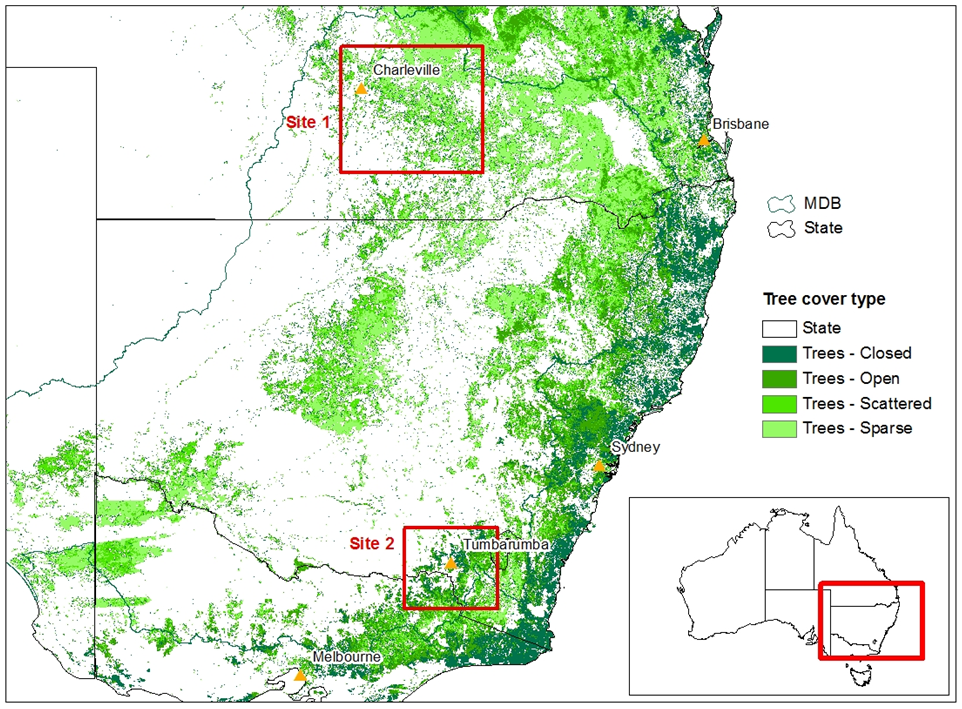
\includegraphics[width=0.9\linewidth]{figures/map_selreg} \caption{Selected study regions are highlighted by red rectangles in the main map (the red rectangle in the insert indicates the location of the main map). The types of tree cover in 2008 from the DLCD product is shown at the background. In site 1 (the QLD region), the tree cover is mostly sparse. In site 2 (the NSW/VIC region), many areas have open or close forest where the tree cover is denser.}\label{fig:selreg}
\end{figure}

Two regions were selected where significant tree cover change since 2000
was reported. The first region is located in south central Queensland
(QLD) partly covering the north of the Murray Darling Basin (MDB) (site
1 in Figure \ref{fig:selreg}). High rates of land clearing have been
reported in this region during the early 2000s (Department of Natural
Resources and Water 2007). The second study region is located at the
border of New South Wales and Victoria (NSW/VIC), and includes the Snowy
Mountain ranges (site 2 in Figure \ref{fig:selreg}). Severe bush fires
occurred in this area in early 2003 (see Figure \ref{fig:bushfire}). The
2003 bush fires were the largest and the worst in the last 60 years (The
State Government of Victoria 2011). Two thirds of Kosciuszko national
park was heavily burned and regrowth was reported to be slow due to
drought and cold conditions (ABC News 2003), and the type of species in
this region. However, in the longer term, after an early high
transpiration period a recovery of pre-fire evapotranspiration would be
expected (Kuczera 1987). For the purpose of this study, significant tree
cover loss has happened in both study areas in the last decade, either
permanently or temporarily.

\begin{figure}
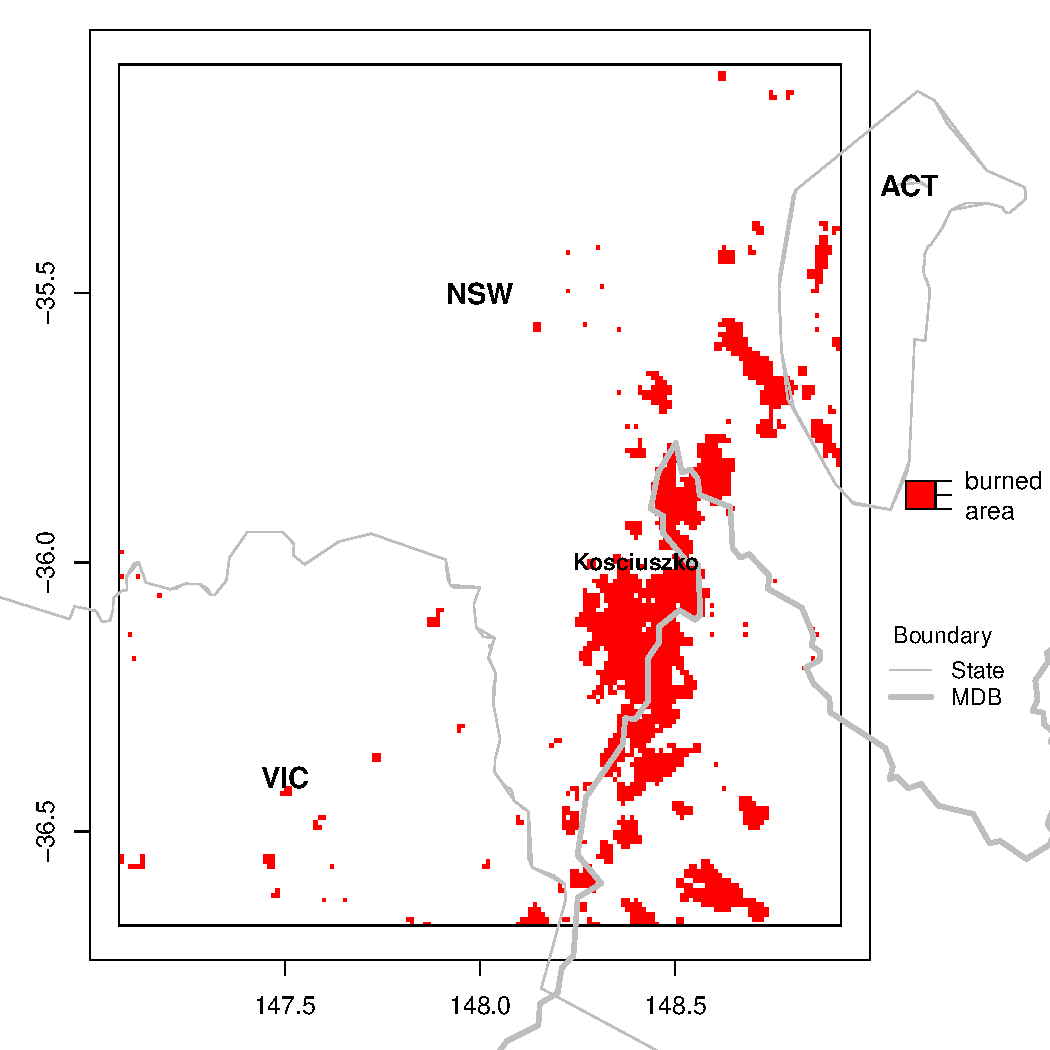
\includegraphics[width=0.9\linewidth]{figures/bushfire_nswvic} \caption{Location of bushfires occurring in January 2003, in and around the NSW/VIC study region, as shown by the red pixels. The map shows the large area in the Kosciuszko national park that has been burned. Some locations in the southwest of the Australian Capital Territory (ACT) have also experienced intensive bushfires.}\label{fig:bushfire}
\end{figure}

The two regions have different characteristics. The QLD region is
partially grassland and subtropical, while the NSW/VIC region is mainly
within the temperate zone, under the Köppen classification. According
to Australian Bureau of Meteorology (BoM), the NSW/VIC region receives
1000 - 2000 mm rainfall annually, which is more than double the annual
rainfall in the QLD region. Evapotranspiration is similar in both
regions. Marine moisture and orographic effects are likely to be the
main contributors to rainfall in the southeast mountain areas of the
NSW/VIC region.

The land use and land cover characteristics in the two regions are also
different. In the Queensland region, the tree cover is sparse over most
of the area. The MODIS satellite tree cover data (discussed in more
detail in section 3) shows that tree cover in this region is generally
below 20\% of total ground area. Grazing is the main activity in this
region, with over 90\% of land used by the grazing industry (ABARES
2010). Our starting assumption is that the main cause of the EVI decline
over large part of the region is due to land clearing. Tree cover has
been cleared at a massive scale over the last decade, especially during
2002 - 2004. The reports from the Queensland Statewide Land Cover and
Trees Study (SLATS) (e.g. Department of Natural Resources and Mines
2005; Department of Science, Information Technology and Innovation 2017)
were used to investigate the time and location of the land clearing in
the QLD region.

The Kosciuszko national park is within the NSW/VIC region. Here tree
cover is denser with open or even closed forest (the tree cover
distribution is bimodal at 10 - 20\% and 60 - 70\%). The dominant
species in the alpine area are Snow Gum and large stand species such as
Alpine Ash and Mountain Gum in the sub-alpine area. These trees can
reach a great height but they take long time to grow. For example,
Alpine Ash would need about 20 years to mature. Although land clearing
is not a major issue in this region, it is vulnerable to fires and
drought. The MODIS burned area product, MCD45A1 (Roy, Lewis, and Justice
2002; Roy et al. 2005; Roy et al. 2008), was used to locate bush fires
areas in the NSW/VIC region, with a grid resolution of 500 m. MCD45A1
provides monthly burning information on all pixels, which helps to
pinpoint an abrupt event.

Due to the difference in nature of the land cover change in the two
regions, the post-change vegetation status is hypothesized to be
different as well (see Figure \ref{fig:figure3-tc-simple}).

\begin{figure}
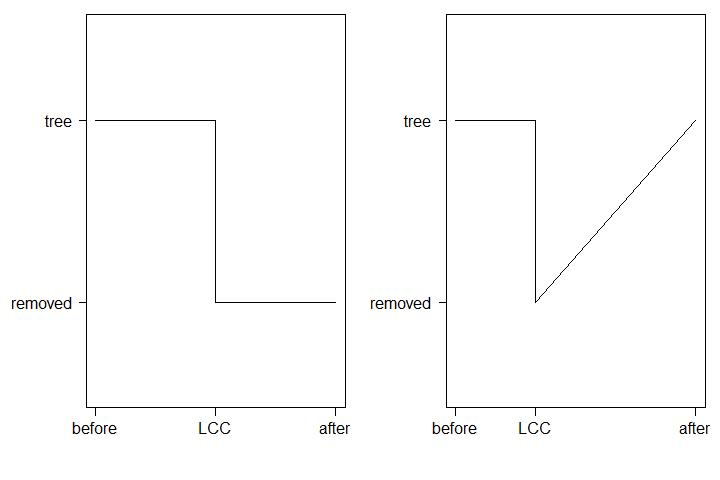
\includegraphics[width=0.9\linewidth]{figures/tc_simple} \caption{The expected evolution of the land surface after trees have been removed in (a) the QLD region and (b) the NSW/VIC region.}\label{fig:figure3-tc-simple}
\end{figure}

The overall hypothesis is that the effect of 2003 - 2004 land clearings
in the QLD region and the 2003 bush fires in the NSW/VIC region cause a
step change in the local rainfall. The actual tree cover change during
this time at the pixel level was derived from the 15-year MODIS data
(discussed below). The difference of tree cover before and after the
land disturbance was tested using a Student's t-test. As the length of
the tree cover data is shorter than available rainfall data, earlier
land clearing in the QLD region cannot be identified spatially, hence
they are excluded from the analysis.

\hypertarget{Data}{\section{Data}\label{Data}}

Several land surface data sets were used in this study. The main one was
the MOD44B product Global Vegetation Continuous Field data set (version
5). This data set provides estimates of percent tree cover (percentage
of ground surface covered by trees) at a grid resolution of 250 m
(Townshend et al. 2011), which is finer than the earlier mentioned
burned product MCD45A1. The data set is available on an annual time
interval for the study period of 2000 - 2015. The tree cover data was
produced from 16-day Terra MODIS Land Surface Reflectance data and Land
Surface Temperature (Townshend et al. 2011). The National Dynamic Land
Cover Dataset (DLCD) (Lymburner et al. 2010) from the Australian
Collaborative Land Use Mapping Program (ACLUMP) was used to verify the
trend of vegetation cover change calculated from the previous data set.
This data set, developed by Geoscience Australia and Australian Bureau
of Agricultural and Resource Economics and Sciences (ABARES), is the
first nationally consistent and thematically comprehensive land cover
reference for Australia. The DLCD is based on the 16-day Enhanced
Vegetation Index (EVI), again from the MODIS satellite, between April
2000 and April 2015. It also has a grid resolution of 250 m. The data
set provides information on the final land cover types (as in 2015) and
estimated trend of EVI statistics (annual mean, maximum and minimum).

The SILO Rainfall product data for Australia was used (Jeffrey et al.
2001) (available online at \url{https://silo.longpaddock.qld.gov.au/}))
. The data has been projected onto a national 0.05\textdegree  by
0.05\textdegree  grid (approximately 5 km by 5 km). This gridded data
set was generated from station observations using spline interpolation
and kriging (Jeffrey et al. 2001). The data has been compared to other
gridded products and observed data and is generally of high quality
(Tozer, Kiem, and Verdon-Kidd 2009; Tozer, Kiem, and Verdon-Kidd 2012).
The data is available on a daily and monthly basis from 1889 to current.
Here a subset of 36 years (1979 - 2015) was used. The study was
conducted on monthly data, as a land cover change effect on annual
rainfall might be negligible, but can often be significant in particular
months or seasons (e.g. Otterman et al. 1990; Gaertner et al. 2001;
Semazzi and Song 2001; Oleson et al. 2004; Deo et al. 2009).

Large scale climate drivers are represented by various climatic indices.
The Southern Oscillation Index (SOI) is generally regarded as a good
predictor of Australian rainfall (Risbey et al. 2009; Chowdhury and
Beecham 2010; Westra and Sharma 2010), but its skill is weaker in some
parts of Australia. For example the Southern Annular Mode (SAM) is found
to be more important than ENSO in south Western Australia (Meneghini,
Simmonds, and Smith 2007). The testing of the suitability of each index
for the regions of interest is described in a later section. The
following climate indices were used as candidate predictors for local
rainfall.

\begin{itemize}
\tightlist
\item
  Southern Oscillation Index (SOI). The Troup version of the monthly SOI
  series used in this study was obtained from BoM (available online at
  \url{http://www.bom.gov.au/climate/current/soihtm1.shtml}).\\
\item
  Eastern, East Central and Central Tropical Pacific Sea Surface
  Temperatures (NINO 3, NINO 3.4 and NINO 4). Monthly SST anomalies are
  available from IRI/LDEO data library and the extended NINO data set is
  used (available online at
  \url{http://iridl.ldeo.columbia.edu/SOURCES/.Indices/.nino/.EXTENDED/}).\\
\item
  Pacific Decadal Oscillation (PDO). The Pacific Decadal Oscillation is
  the leading principal component of monthly SST anomaly in the North
  Pacific Ocean.. The monthly PDO series was provided by JISAO (Joint
  Institute for the Study of the Atmosphere and Ocean, University of
  Washington) (available online at
  \url{http://jisao.washington.edu/pdo/PDO.latest}).\\
\item
  Indian Ocean Dipole (IOD). The Indian Ocean dipole is commonly
  measured by the difference between SST anomaly in the western (50 -
  70\textdegree E and 10\textdegree S-10\textdegree N) and eastern (90 -
  110\textdegree E and 0 - 10\textdegree S) equatorial India Ocean (Saji
  et al. 1999). Monthly IOD was obtained from JAMSTEC (the Japan Agency
  for Marine-Earth Science and Technology) (available online at
  \url{http://www.jamstec.go.jp/frcgc/research/d1/iod/DATA/dmi.monthly.txt}).
\end{itemize}

\section{Statistical method}\label{statistical-method}

As an initial analysis a simple boxplot and t-test is used to analyse
whether there is a significant change in tree cover in time, and before
and after the suspected change in the regions.

To assess the actual causal relationship between the tree cover and the
rainfall a flexible regression model is applied (discussed in detail
below). A step change is not directly obvious in the time series of the
rainfall anomalies (Figure \ref{fig:ts-mean}) for both regions, even
though the data is deseasonalised and detrended. In this study we apply
different statistical methods to analyse the effect of tree cover change
on rainfall. Both methods make use of a regression model to remove
year-on-year variability in rainfall to strengthen the tree cover change
signal.

In the first method, the tree cover change is implemented as a factor
variable in the regression model, and the significance of this variable
is tested. In the second method, a rank sum test (step trend test), is
applied to the regression model residuals after effects of other major
factors were removed. This assumes that after removal of all climate,
long term linear trend and seasonal variation, the vegetation cover
change is the only factor explaining the non-random pattern in the
rainfall residuals.

\begin{figure}
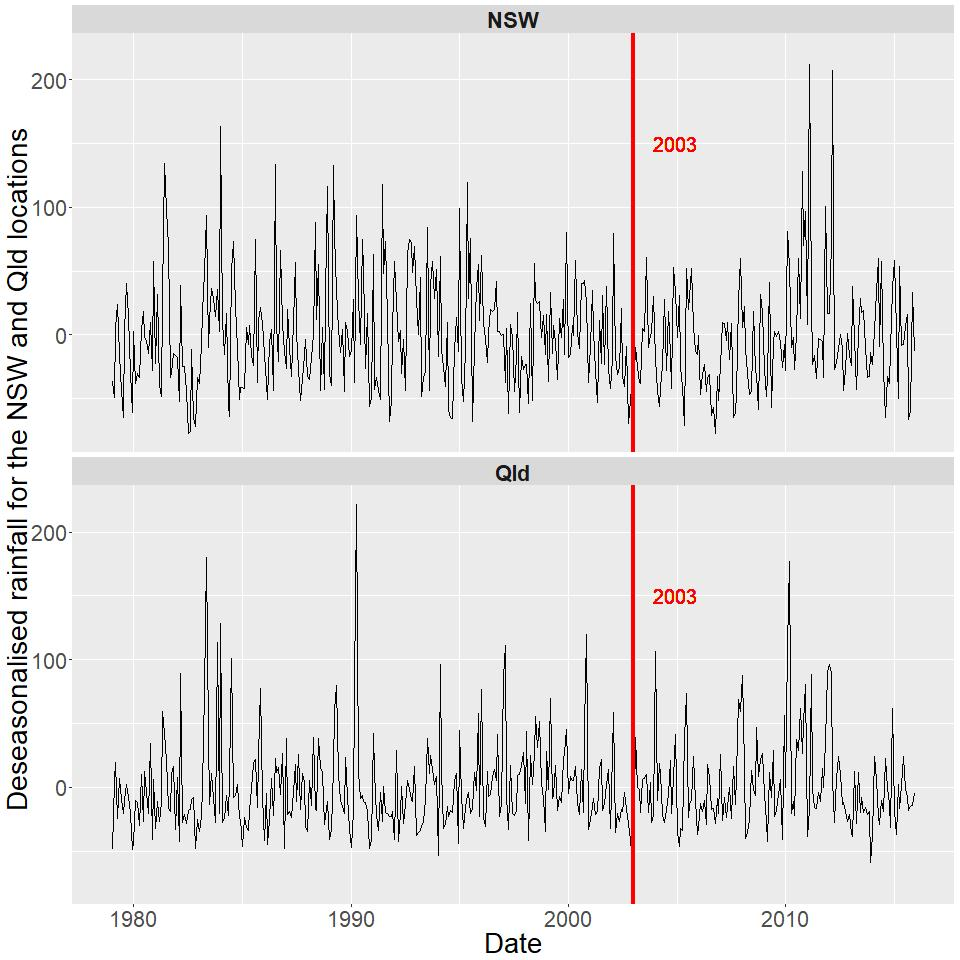
\includegraphics[width=0.9\linewidth]{figures/Rainfall_resid} \caption{The deseasonalised and detrended rainfall over the 30 years period in (a) the QLD region and (b) the NSW/VIC region. The vertical red lines indicate the year of 2003, in which the studied land cover changes occurred. A change in the time series data is not obvious before and after the land cover changes.}\label{fig:ts-mean}
\end{figure}

\subsection{Regression model}\label{reg_model}

As highlighted in the introduction, the Australian climate is influenced
by sea surface temperatures in the tropical Pacific and Indian Oceans,
as well as pressure systems in the Southern Ocean (BoM 2012b). Risbey et
al. (2009) compared five large-scale drivers, including ENSO (measured
by SOI and the Tropical Pacific Sea surface temperatures (SSTs)), IOD,
SAM, MJO (Madden-Julian oscillation) and blocking, in relation to
Australian rainfall variability. The MJO is a large scale
eastward-propagating wave-like disturbance located around equatorial
latitudes (Risbey et al. 2009). They identified SOI as the most
important index among all climate indices tested for broad parts of
Australia (including QLD and NSW/VIC) in almost any season. In this
study, four climate indices were selected from the main climatic
indicators (see section \protect\hyperlink{Data}{Data}) and used as the
explanatory variables in the model for each study region. A further
complicating factor is the influence of the ``millenium drought'' over
the study period and in particular the change to wet conditions in 2010
- 2011 (Dijk and Viney 2013). Therefore, the spatially averaged monthly
rainfall in the Murray Darling Basin (MDB, downloaded from
\href{http://www.bom.gov.au/web01/ncc/www/cli_chg/timeseries/rain/allmonths/mdb/latest.txt}{the
Bureau of Meteorology}) was used to explain the year-on-year variation
in the rainfall in the regions. As climate alone are unlikely able to
fully explain the temporal variation in rainfall in the regions,
including the drought (Dijk and Viney 2013; Westra and Sharma 2010),
this variable was included. Since both regions at least partly overlap
with the MDB, the average rainfall for the entire basin was assumed to
be a useful explaining variable.

Correlations between rainfall and each climate index were analysed.
Rainfall in each study region was first deseasonalised and detrended
using the seasonal decomposition function \texttt{ds} in the package
\texttt{deseasonalise} in R (R Core Team, 2018). Using detrended data
gives a better indication of the underlying correlation by removing the
underlying correlation in the data (Smith and Timbal 2012). The
cross-correlations between the deseasonalised and detrended rainfall and
the climatic indices were tested using the Pearson's product moment
correlation method, assuming the relationships are linear. Although the
optimal technique for exploring the correlation with each index could be
different as described in Risbey et al. (2009), the Pearson's method was
applied to all indices for consistency. Because the PDO describes the
multi-decadal SST with lower frequency (MacDonald and Case 2005;
Zanchettin et al. 2008; Kamruzzaman, Beecham, and Metcalfe 2011),
instead of 37-year rainfall data, a longer period (115 years, from 1900
to 2015) was used to estimate the correlation with PDO, up to lag 24.
For the other indices, the 37-year data was used.

\begin{figure}
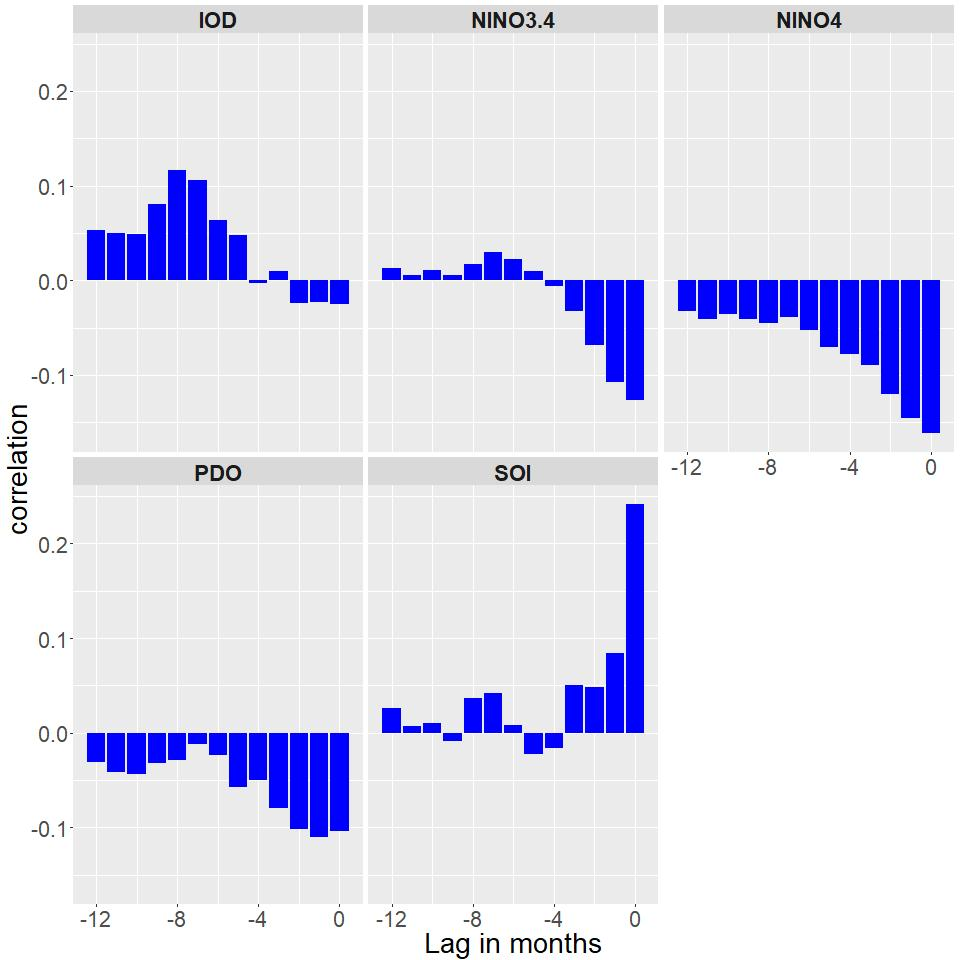
\includegraphics[width=0.9\linewidth]{figures/cor_qld} \caption{Cross-correlation of six climate indices and rainfall in QLD study region. For the PDO analysis, 108-year rainfall data (1900 - 2008) are used. Otherwise, 36-year rainfall data are used. The correlation with NINO 3 is not shown as it is very similar to but weaker than for NINO 3.4.}\label{fig:cor-rain-qld}
\end{figure}

\begin{figure}
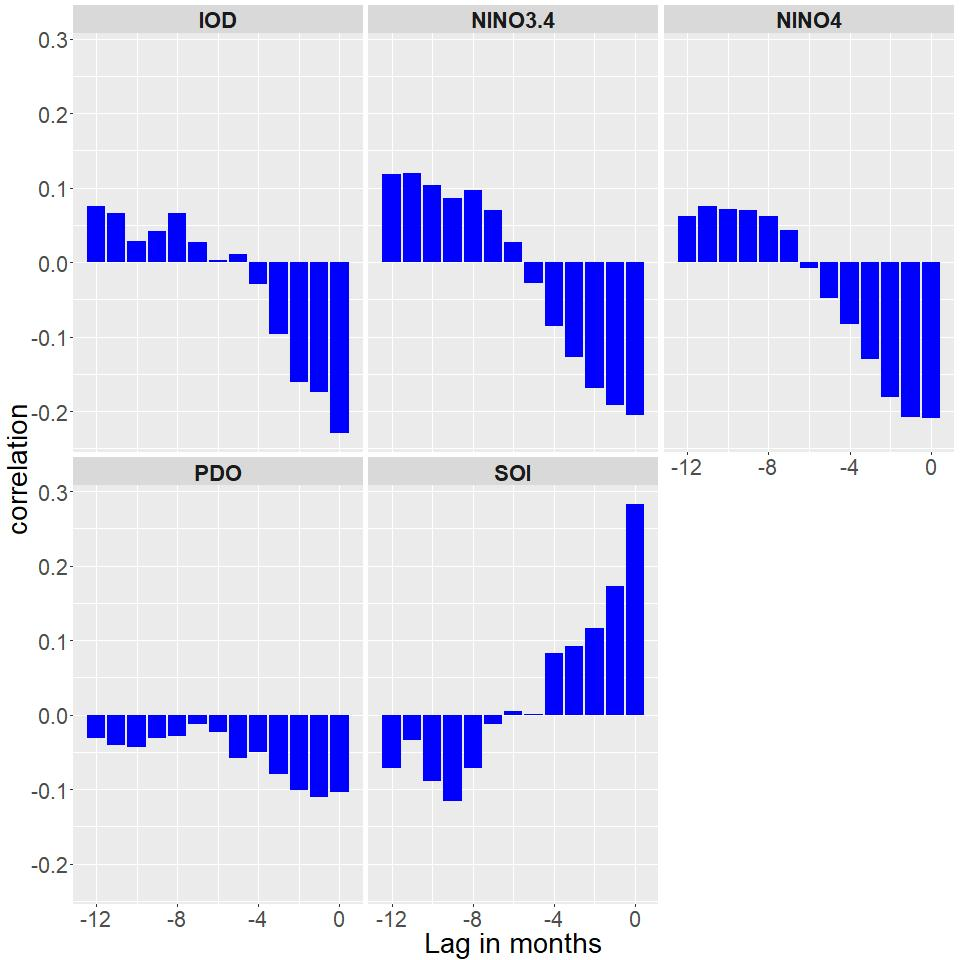
\includegraphics[width=0.9\linewidth]{figures/cor_nswvic} \caption{Cross-correlation of six climate indices and rainfall in NSW/VIC study region.}\label{fig:cor-rain-nsw}
\end{figure}

Based on the correlation between the climatic indices and rainfall in
the regions (as shown in Figure \ref{fig:cor-rain-qld} and Figure
\ref{fig:cor-rain-nsw}), it can be concluded that:

\begin{itemize}
  \setlength{\itemsep}{0cm}
  \setlength{\parskip}{0cm}
  \item In QLD, the correlation between rainfall and SOI at zero time lags is the strongest across all indices, outweighing the other ENSO indicators. IOD and PDO have a weak influence in QLD.
  \item In NSW/VIC, again the SOI has the strongest correlation with rainfall, followed by the IOD. For both, the strongest correlations occur at the zero time lags. 
  \item In both cases PDO had the weakest correlations, and this factor was not further considered as a predictor.
  \item In general, for the better correlated indices, strongest correlations occured at zero time lags.
\end{itemize}

The above findings are consistent with previous studies. Although some
indices are serially correlated with rainfall up to several months, the
lag zero events have the greatest correlation coefficients. Using
multiple climatic index series was generally found most useful in
rainfall prediction (e.g. Risbey et al. 2009; Kamruzzaman, Beecham, and
Metcalfe 2011).

Rainfall in Australia shows strong seasonal patterns (Holper 2011;
Australian Bureau of Statistics 2012). For example, the north part of
the country is summer rainfall dominant with a dry winter, while most of
the southern part has a winter rainfall regime. This character is driven
by the movement of subtropical high pressure systems which dominate the
Australian climate (BoM 2012a). These characteristic summer and winter
rainfall patterns mean that the seasonal component of rainfall has a
periodic pattern which should be included in the model.

Long term trends in the regional rainfall in some parts of Australia are
significant (Hughes 2003; Gallant, Hennessy, and Risbey 2007; Chowdhury
and Beecham 2010). In the northern and eastern parts of the continent,
increasing rainfall is reported over the last century (Hughes 2003). The
presence of such long term trends may be confused with the outcome of a
step change in rainfall. As a result a linear trend term was implemented
in the model to remove any long term effect.

We assumed all the factors are additive smooth components in determining
rainfall following Kamruzzaman, Beecham, and Metcalfe (2011). In this
case, the rainfall model is a generalised additive model (GAM) (Hastie
and Tibshirani 1986) with a log link function \texttt{g()} and assuming
the residuals are gamma distributed (see Figure \ref{fig:hist-rain}).
This means all predictors are modelled as smooth functions, in this case
using the shrinkage version of the cubic regression splines (Wood 2011).
All splines were limited to 3 knots in flexibility (Wood 2011), to
reduce the risk of overfitting. \vspace{0.5cm}

\begin{equation}
\begin{array}{lll}
g(E(\mathbf{R}_r)) = &\beta_0 + s_1(\mathbf{MDB_{monthlyRain}} + s_2(\mathbf{SOI}) + s_3(\mathbf{IOD}) + \\
&s_4(\mathbf{Nino3.4}) + s_5(\mathbf{Nino4}) + s_6(\mathbf{Season}) + \\
           &\beta_1\mathbf{Trend} + \boldsymbol{\epsilon}_r
\end{array}
\label{eq:model}
\end{equation}

The bold letters represent the time series vectors. The region is
indicated by \(r\), while \(\beta_u\) (\(_u\)=0, 1) are the fitted
coefficients in the model. \(s_v\) (\(_v\)=1, 2, 3,\ldots{}) are the
smooth penalized cubic regression spline functions on the climatic
indices and the season. MDB\textsubscript{monthlyRain} is the spatially
averaged monthly rainfall across the Murray Darling Basin. Apart from
dropping PDO as a predictor, all other climate indices were included,
allowing the model to select the appropriate predictors.

A possible linear long term trend in the rainfall data is modelled by
\textbf{Trend} = 1,2,3\ldots{}n, where n is the total number of months
in the time series. \textbf{Season} is the seasonal component. The
climatic terms are also modelled with smooth functions. The effect of
large scale drivers on Australian rainfall is more likely to be seasonal
(Murphy and Timbal 2008; Schepen, Wang, and Robertson 2012), and the
smooth spline function is more flexible in reproducing the variability
in impacts of the climatic indices.

\begin{figure}
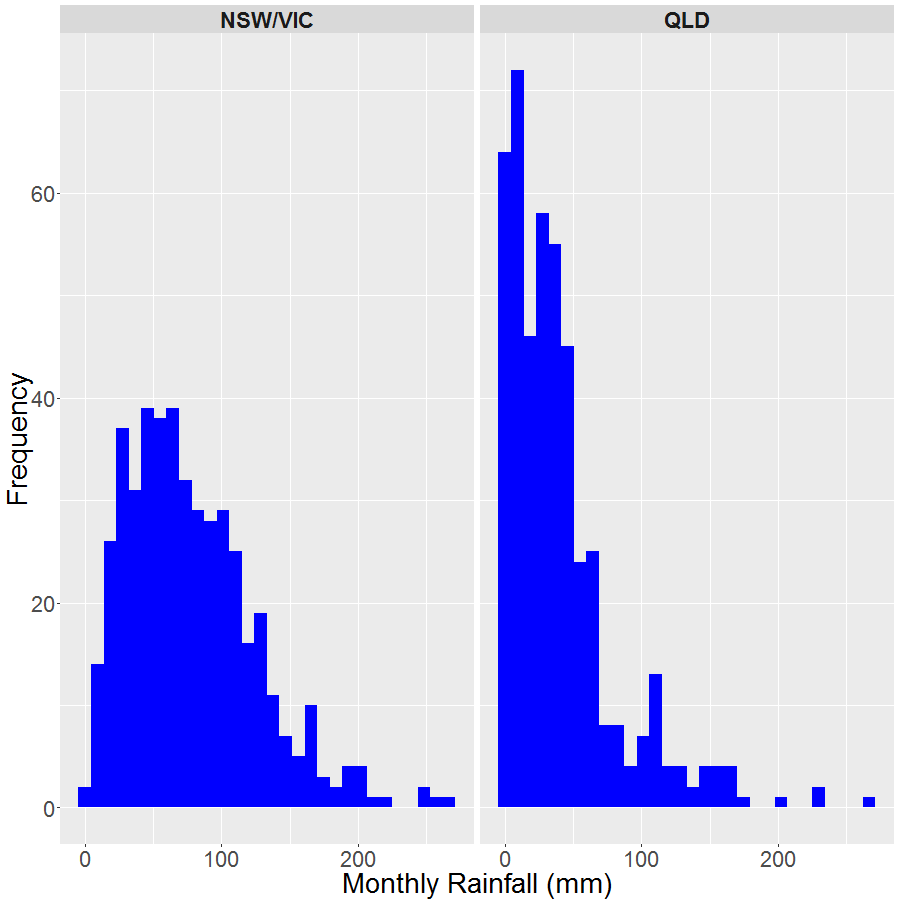
\includegraphics[width=0.9\linewidth]{figures/hist_rainfall} \caption{Distribution of monthly rainfall in (a) QLD and (b) NSW/VIC. Using a Kolmogorov-Smirnov test with shape = 1 and 2.4  for QLD and NSW/VIC respectively, rainfall in both regions can be modelled as a gamma distribution.}\label{fig:hist-rain}
\end{figure}

\subsection{Tree cover change as factor variable}

One of the main difficulties in empirical observation studies related to
the effect of land cover change on rainfall is the lack of continuous
monitoring of land surface variables. Moreover, no specific variable can
possibly be defined that can clearly represent the land surface process.
Given the lack of a full picture of the land surface process, a factor
variable was used in the regression model to represent the abrupt land
surface change (see Equation \eqref{eq:model}). The change could be a
result of either land clearing or bush fires as long as it is permanent
or takes a long time to recover. As indicated we approached the problem
in two different models ways.

In the first method, the tree cover change was used as a predictor in
the regression model, represented by a factor variable \textbf{LC}. The
significance of the coefficient of \textbf{LC}, denoted as \(\beta'_5\)
in Equation \eqref{eq:model}, can be determined by a ratio test.

\begin{equation}
  \mbox{LC} = \left\{
  \begin{array}{ll}
     \mbox{Trees} \\
     \mbox{Removed}
  \end{array} \right.\\
\label{eq:dummyC}
\end{equation}

Therefore in both regions, land cover is ``trees'' for the period before
land cover change and ``removed'' for the period after the change. Here
we simply assumed that vegetation cover change has occurred on every
pixel. The remaining term \(\epsilon_r\) is the amount of rainfall that
is attributed to other unspecified factors and random errors. Hence the
regression model becomes \vspace{0.5cm}

\begin{equation}
\begin{array}{lll}
g(E(\mathbf{R}_r)) = &\beta'_0 + s'_1(\mathbf{MDB_{monthlyRain}} + \\
  &s'_2(\mathbf{SOI}) + s'_3(\mathbf{IOD}) + \\
  &s'_4(\mathbf{Nino3.4}) + s'_5(\mathbf{Nino4}) + s'_6\mathbf{Season} + \\
  &\beta'_1\mathbf{Trend} + \beta'_2\mathbf{LC} + \boldsymbol{\epsilon'}_r
\end{array}
\label{eq:model2}
\end{equation}

One of the difficulties is to point an exact time to the changes in the
vegetation cover in the two regions. In the QLD region, no exact time
can be assigned to the land clearing. According to the SLATS reports,
the most substantial clearing occurred between 2003 - 2004 . However,
the information on the change in type of land cover during the time
period is missing. Therefore, four scenarios were initially tested in
the analysis, however there was no real difference between these
scenarios. In the NSW/VIC region, severe bush fires were reported in
early January 2003. Hence the ``tree'' cover state was up to December
2002 then it was changed to ``removed'' state from January 2003. As a
starting date, the regression model was run from 1979 for both regions.

\subsection{Step trend test}\label{step-trend-test}

To support the regression analysis, a Mann-Whitney Rank-Sum step trend
test was used to detect changes in rainfall as a result of vegetation
cover change. This specific nonparametric statistical test was modified
from the Mann-Whitney U test by Hirsch and Gilroy (1985) and can
identify a step change in data which is cross-correlated. The gridded
rainfall dataset used in this study has a high spatial correlation
between neighbouring pixels due to the underlying interpolation method.
The advantages of using the Rank-Sum test are: (1) it does not depend on
assumptions of the data distribution; (2) it is not restricted to
datasets with no missing data; (3) it is robust and not as easily
influenced by outliers and negative numbers (Hirsch and Gilroy 1985).
However, the test has less power than parametric tests.

The rainfall residuals from the regression model in Equation
\eqref{eq:model2} were used for the step trend test. To detect a step
change, using deseasonalised and detrended data is important (Hirsch and
Gilroy 1985). Furthermore, as rainfall can only be partially attributed
to local sources and conditions, other effects are introduced by large
scale dynamics and changes in climatic factors. The assumption is that
the regression model should remove these effects, and additionally
deseasonalise and detrend the rainfall data. As a result, the local
landuse effects are amplified in the remaining residuals. The test,
described in the following sub section, subsequently associates trends
in the rainfall residuals with tree cover changes.

\subsubsection{Mann-Whitney rank-sum
statistic}\label{mann-whitney-rank-sum-statistic}

As indicated, the step trend test is a modified version of the
Mann-Whitney U statistic (Hirsch and Gilroy 1985). As a nonparametric
rank-based test, the Mann-Whitney test does not use the exact values of
rainfall but depends on the ranks of the data. For each month, rainfall
residuals of each year were ranked in an ascending order. The ranking of
January rainfall in a sample pixel k in QLD is illustrated below:

\begin{table}[t]

\caption{\label{tab:exampleRank}Example of ranking rainfall residuals}
\centering
\begin{tabular}{rrr}
\toprule
Year & Rainfall residuals & Rank \$R'\_\{1k\}\$\\
\midrule
1998 & -0.3 & 6\\
1999 & -60.9 & 2\\
2000 & -16.1 & 4\\
2001 & -71.7 & 1\\
2002 & 111.1 & 7\\
\addlinespace
2005 & -7.2 & 5\\
2006 & -60.5 & 3\\
\bottomrule
\end{tabular}
\end{table}

\noindent Therefore, the smallest or most negative value has rank 1 and
the largest value has the maximum rank.

The before and after period in the data formed two groups of samples.
The split point of the two periods was based on the timing of the
vegetation cover changes. In the QLD region, changes occurred anytime
during 2003 and 2004. In contrast to the previous method, the time
period covering the land cover change was excluded, as the nonparametric
test allows missing data. Hirsch and Gilroy (1985) also pointed out that
the power of the test is higher if the data of the change period is
ignored. Hence 2003 and 2004 were excluded from the analysis. As a
result, the post change period was 2005 - 2015 for the Queensland
location.

In the case of NSW/VIC, the bushfires broke out in early January 2003.
The change was within a relatively short period of the year. Therefore
the post change period in this region still started in January 2003.
Following Hirsch and Gilroy (1985), the pre change period was set to
five years (1998 - 2002) in both regions. The length of the post change
period is also difficult for the NSW/VIC region, as the regrowth would
at some point have impacted the local effects.

The rank of rainfall in month j year i in pixel k is denoted as
\(R'_{ijk}\). The sum of ranks of rainfall in month j in pixel k before
the known intervention is:

\begin{equation}
  W_{jk} = \sum_{i=1}^{n_1}R'_{ijk}.
  \label{eq:Wj}
\end{equation}

\(n_1\) is the number of years before the land cover change. The
expected value of \(W_{jk}\) is

\begin{equation}
  \mu_w=n_1(n_1+n_2+1)/2
\end{equation}

\(n_2\) is the number of years after the change. Hence the expected
value of the rank sum before the intervention is the same for all months
and all pixels. The sum of ranks for the whole time period is fixed, as
\((n_1+n_2)(n_1+n_2+1)/2\). In this study, since there are only two
groups (before and after), knowing the rank-sum of one group is the same
as knowing the rank-sum of the other group. If the rainfall data is
temporally and spatially independent, the variance of \(W_{jk}\) is

\begin{equation}
  \sigma^2_w = n_1\cdot n_2(n_1+n_2+1)/m
\end{equation}

where m is the number of months which is 12 in the case of a full year.

\subsubsection{Step trend test}\label{step-trend-test-1}

Instead of completing the Mann-Whitney U-test, Hirsch and Gilroy (1985)
applied a standard normal Z test to the rank-sum statistics. As
highlighted, this modified test accounts for serial temporal
autocorrelation and spatial cross correlation in the data. In the case
here, the deseasonalised and detrended data shows little autocorrelation
in the time series but possesses strong cross correlation between
neighbouring pixels, i.e. \(R>0.99\).

The sum of \(W_{jk}\) for a block of \(ns\) pixels over the whole year,
\(\sum_{j=1}^{12}\sum_{k=1}^{ns}W_{jk}\), has mean

\begin{equation}
  E(\sum_{j=1}^{12}\sum_{k=1}^{ns}W_{jk})=12\cdot ns\cdot\mu_W
\end{equation}

and variance

\begin{equation}
  Var(\sum_{j=1}^{12}\sum_{k=1}^{ns}W_{jk})=\sum_{j=1}^{12}\sum_{k=1}^{ns}\sum_{h=1}^{ns}C(W_{jk},W_{jh}).
\end{equation}

\(C(W_{jk},W_{jh})\) is the covariance of the W statistics between pixel
k and pixel h in month j. When \(k=h\), \(C(W_{jk},W_{jh})=\sigma^2_w\).
When \(k\neq h\),

\begin{equation}
  C(W_{jk},W_{jh})=\sigma^2_w r(R_k,R_h)
\end{equation}

where \(r(R_k,R_h)\) is the product moment correlation coefficient of
the concurrent ranks in pixel k and h. Here \(r\) is calculated on the
full time series in each pixel. In the analysis, the test was applied to
a square block of four pixels each time. As argued by Hirsch and Gilroy
(1985), \(ns=4\) is the most optimal solution to balance the cost and
the gain in the test power.

The statistic of the step trend test is then defined as

\begin{equation}
  Z'=\frac{\sum_{j=1}^{12}\sum_{k=1}^{ns}W_{jk}-12\cdot ns\cdot\mu_w}{\sqrt{Var(\sum_{j=1}^{12}\sum_{k=1}^{ns}W_{jk})}}.
  \label{eq:Z}
\end{equation}

The above statistic is written for a 12 month period. By changing the
value 12, it can also be used to test seasonal rainfall change or for
other customized periods.

\begin{table}[t]

\caption{\label{tab:Zscore}The interpretation of Z' score in the step trend test}
\centering
\begin{tabular}{l}
\toprule
 \\
\midrule
$Z'>0$  and rainfall decreases after change\\
$Z'<0$ and rainfall increases post change\\
$Z'=0$ and rainfall does not change\\
\bottomrule
\end{tabular}
\end{table}

The null hypothesis (\(H_0\)) in this study is that there was no change
in rainfall due to land surface intervention. The results of the step
trend test can be interpreted according to the sign of the Z' score (see
Table \ref{tab:Zscore}, Chapter 23, P887 (Hipel and McLeod 1994)). Z' is
normally distributed similar to the standard normal statistics Z. Hence
it can be compared to a standard normal distribution to determine the p
value.

\section{Results}\label{results}

\subsection{Tree cover change}\label{tree-cover-change}

The pixels, where the tree cover change based on the MOD44B data was
significant (\(p \leq 0.05\)) in each study region, are shown in Figure
\ref{fig:tctrend} for the NSW/VIC region (left panel) and the QLD region
(right panel). In the QLD region there actually has generally been an
increase in tree cover after the clearing of native vegetation stopped.
In the NSW/VIC region, much of the tree loss between 2002 and 2003 was
concentrated in the Snowy Mountains close to the border of NSW and VIC,
which is also evident in the figure. Tree cover loss occurred in large
parts of the QLD region between 2002 and 2005, but this tree loss was
spatially less concentrated.

\begin{figure}
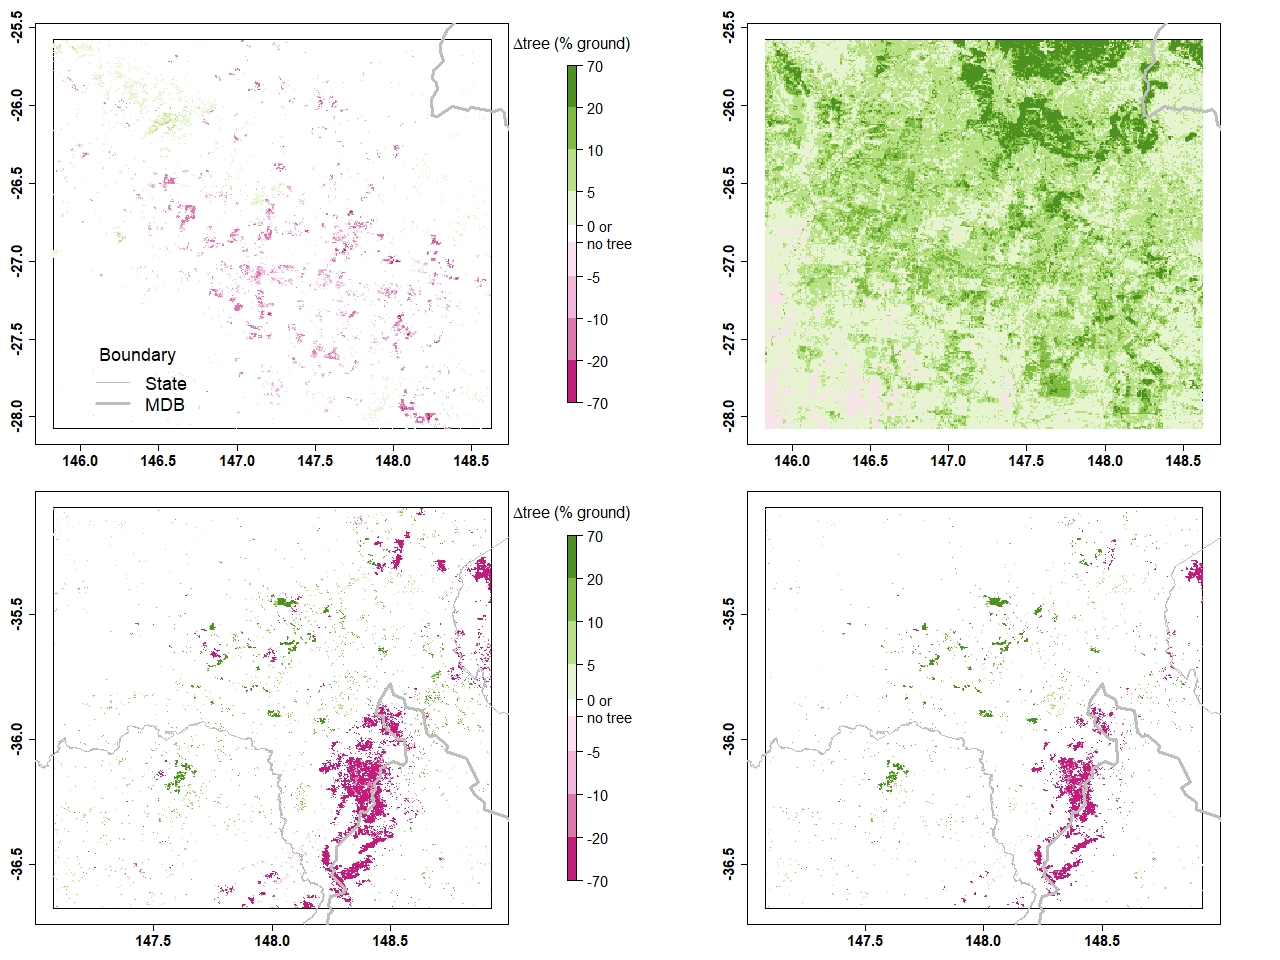
\includegraphics[width=0.9\linewidth]{figures/tc_figs} \caption{The maps show significant changes in tree cover identified from the MOD44B data between 2003 and 2015 in the NSW/VIC region (right) and the Qld region (left). The amount of change was calculated as the difference in tree cover before and after the specified land cover intervention and it is shown as the percentage of the ground area. Green colour indicates an increase in tree cover, while red colour indicates a decrease in tree cover.}\label{fig:tctrend}
\end{figure}

\subsection{Regression Model and significance of Vegetation Cover
Changes}\label{regression-model-and-significance-of-vegetation-cover-changes}

\begin{figure}
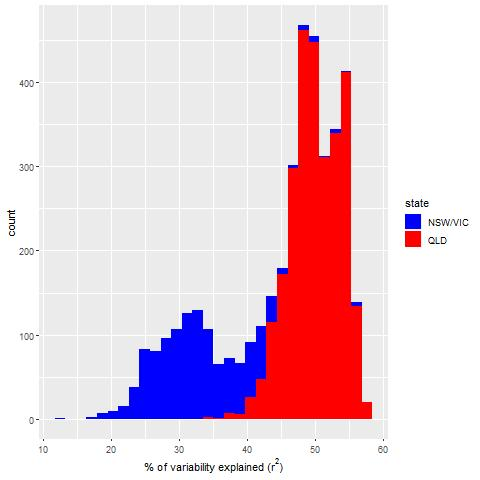
\includegraphics[width=0.9\linewidth]{figures/rsq_fullmodel} \caption{The distribution of the variance explained (adjusted $r^2$ ) by the full regression model}\label{fig:rsqmodel}
\end{figure}

Generally the regression model only explains a limited amount of the
rainfall variability (Figure @reg(fig:rsqmodel)). The model in Equation
\eqref{eq:model2} accounts for an average around 33\% of the variation in
the NSW/VIC region and about 50\% of the variation in the QLD region as
indicated by the adjusted \(r^2\). The adjusted \(r^2\) is the
coefficient of determination, a measurement of the amount of variability
predicted by the model adjusting for the number of explanatory terms.
The residual analysis shows that the assumptions of the regression model
are generally met (Figure \ref{fig:residuals}). The standardised
residual plots, however, show some funnelling for the NSW/VIC regions,
suggesting non constant variance. The residual patterns are consistent
for all pixels within each region.

In terms of predictors of the local rainfall in the model, logically,
the average rainfall across the larger Murray Darling Basin is highly
significant. This confirms that this variable is a good reflection of
the year on year variability in the rainfall. The model also confirms
the importance of the climate drivers and the seasonality in Australian
rainfall, as many of these variables were significant. Even at the grid
level, the seasons and several of the climatic indices were significant
(\(p \leq 0.05\)) everywhere in both regions. The climate drivers (at
lag zero) accounted, on average, for 6.5\% of the rainfall variability
in both the QLD region and the NSW/VIC region (see Figure \ref{fig:rsq}
for the distribution of adjusted \(r^2\) in these two regions). These
figures are within the upper bound of seasonal rainfall predictability
by a SST anomaly field reported by Westra and Sharma (2010).

\begin{figure}
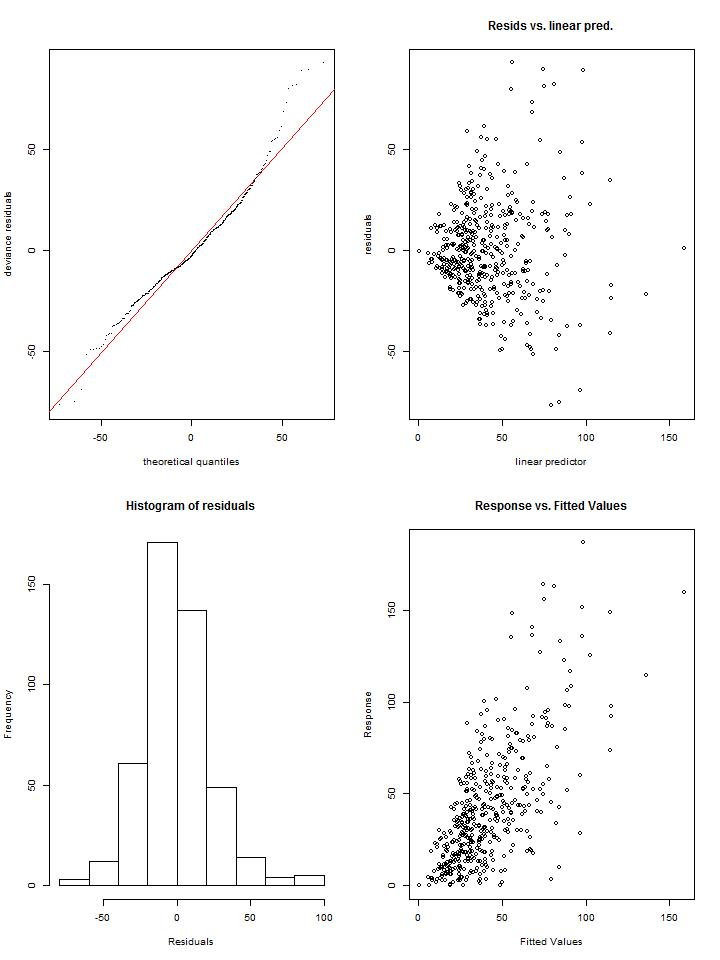
\includegraphics[width=0.9\linewidth]{figures/gam_check} \caption{The residual analysis of a sample pixel in the QLD region (top) and NSW/VIC region (bottom).}\label{fig:residuals}
\end{figure}

\begin{figure}
\includegraphics[width=0.7\linewidth]{figures/soi_explhistogram} \caption{The performance of the regression model if rainfall is only modelled by the climate drivers. It shows the percentage of rainfall variability that can be explained by the climate drivers for the Qld and NSW/VIC region}\label{fig:rsq}
\end{figure}

There were generally no statistically significant long term trends in
both regions. However, this result might not prove or disprove the
existence a long term trend in rainfall. The overall time period is
fairly short (Koutsoyiannis 2006) and more pixels in NSW/VIC could
indicate a significant step change if the long term trend effect is not
removed by the model. As trend free data is an important requirement for
the step trend test, the trend term was kept in the regression model to
ensure the detection of step change was not due to a possible long term
trend.

\begin{figure}
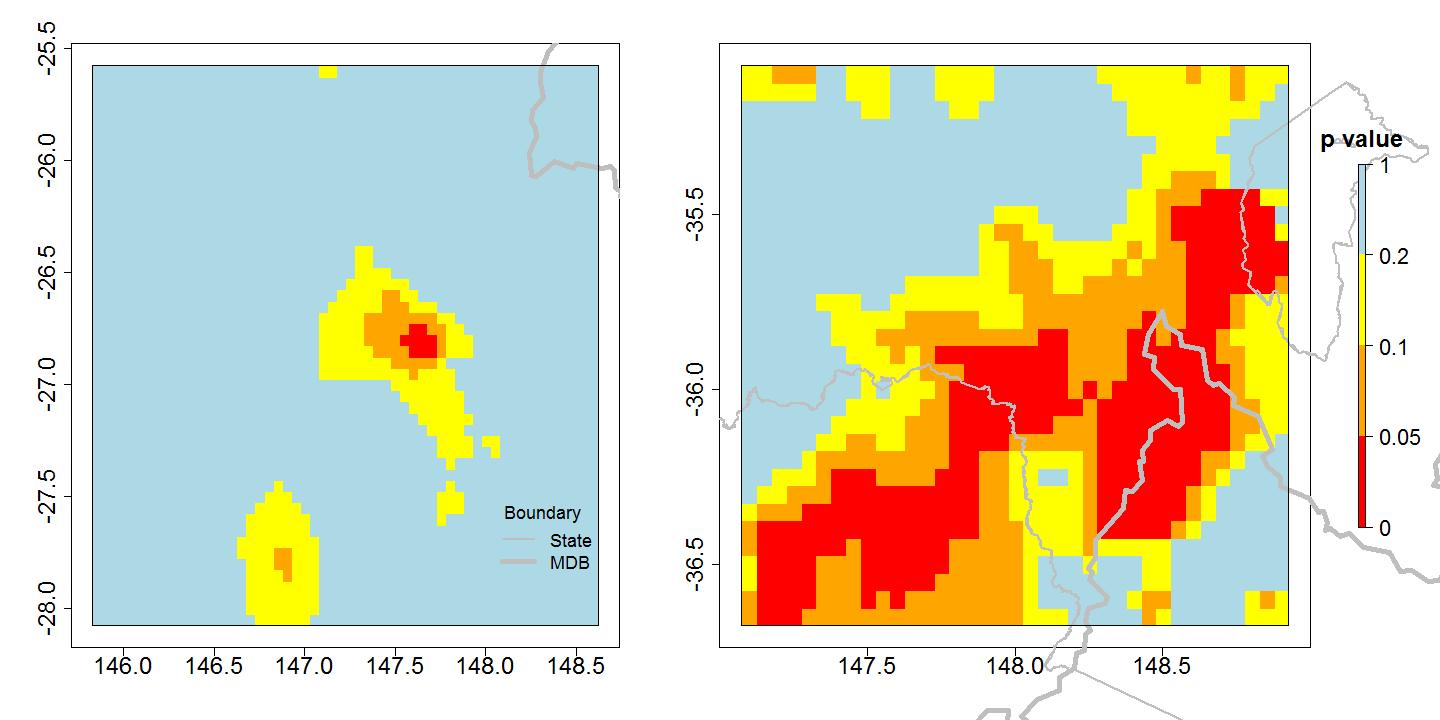
\includegraphics[width=0.9\linewidth]{figures/Cp_30yrs} \caption{The spatial distribution of significance of land cover step change variable in the GAM model predicting changes in rainfall in the both regions. The left graph relates to the Qld region, while the right hand plot reflects the NSW/VIC region. The outlines of relevant Australian states and the Murray Darling Basin are indicated in grey.  The p value reported is for the land cover variable in the model.}\label{fig:LCp}
\end{figure}

The land cover variable in the model (Equation \eqref{eq:model2}) aims to
identify a step change in the rainfall before and after the observed
change in land cover. The variable was mainly significant
(\(p \leq 0.05\)) for the rainfall estimates in some areas in NSW/VIC,
as shown in Figure \ref{fig:LCp} (right panel). However, the number of
pixels where the landcover variable was significant was much greater in
NSW/VIC compared to the QLD region. There was also some relationship
between the areas of bushfires in Figure \ref{fig:bushfire}. Only a very
small area with a significant step change due to the land cover changes
was found in rainfall in the QLD region (left panel)

More generally, the model for NSW/VIC suggests that the land cover
variable has a positive impact on rainfall in both regions. The fitted
coefficients for the Land cover change variable were consistently
positive for the ``tree'' part of the series. It implies that rainfall
was higher when the surface was covered by trees.

\subsection{Step Trend Test}\label{step-trend-test-2}

\begin{figure}
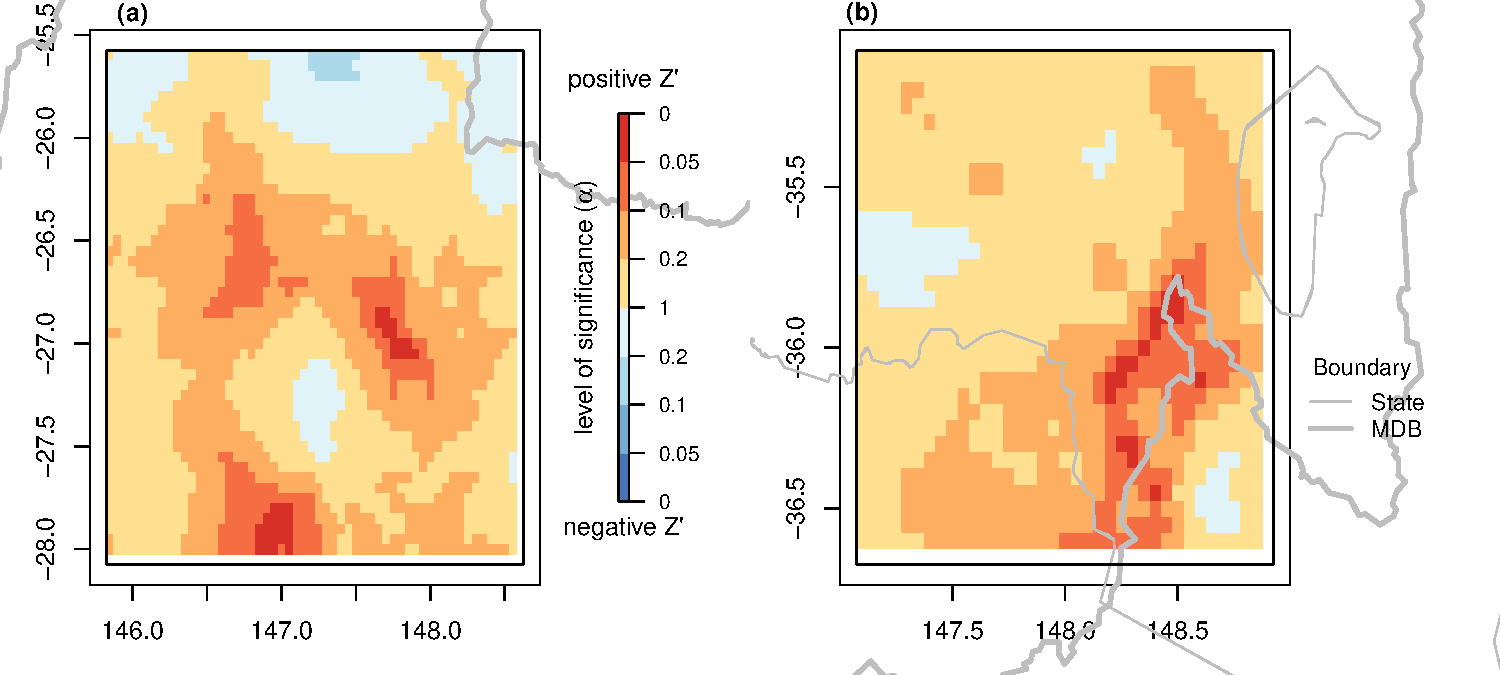
\includegraphics[width=0.9\linewidth]{figures/step_new} \caption{Spatial distribution of the step trend test Z' statistics in the two study sites. The panel on the left is for the QLD region, while the panel of the right is for NSW/VIC. Warm colours (yellow, orange and red) are for positive Z' values which indicate decreasing rainfall trend due to the land surface change. Cold colours (light blue to blue) are for negative Z' values which indicate increasing rainfall trend. The deeper the colour, the more significant the statistic.}\label{fig:steptest30}
\end{figure}

The spatial step trend test based on the regression residuals without
the landcover variable generates Z' scores. The results for the Qld
region (left) and NSWVIC region (right) are shown in Figure
\ref{fig:steptest30}. This figure provides two types of information: the
sign and the significance level. The sign indicates the direction of the
step change in the residuals of the regression, as listed in Table
\ref{tab:Zscore}. In both regions there are areas of positive Z' values
which imply a decrease in rainfall, but this is stronger in the NSW/VIC
area than in the QLD area. For the NSW/VIC area there appears to be a
reasonable relationship between the locations where changes in tree
cover are observed (Figure \ref{fig:tctrend}) and the patterns in the Z'
score. However, there is not necessarily a direct relationship as
movement of air masses could mean that actual changes of rainfall are
observed close by, but not necessarily exactly at areas with changes of
landcover. There is once again a difference between the left panel and
the right panel, indicating only a few significant of Z' scores in the
QLD region wich matches the earlier significance in the landcover
variable in the full regresion. In the QLD region, only 0.2\% of the
pixels obtained a positive Z' score with p \(<\) 0.1. In the NSW/VIC
region 3.7\% of pixels have a positive Z' score with p \(<\) 0.1. In
general it is only a small proportion of both study regions.

\begin{figure}
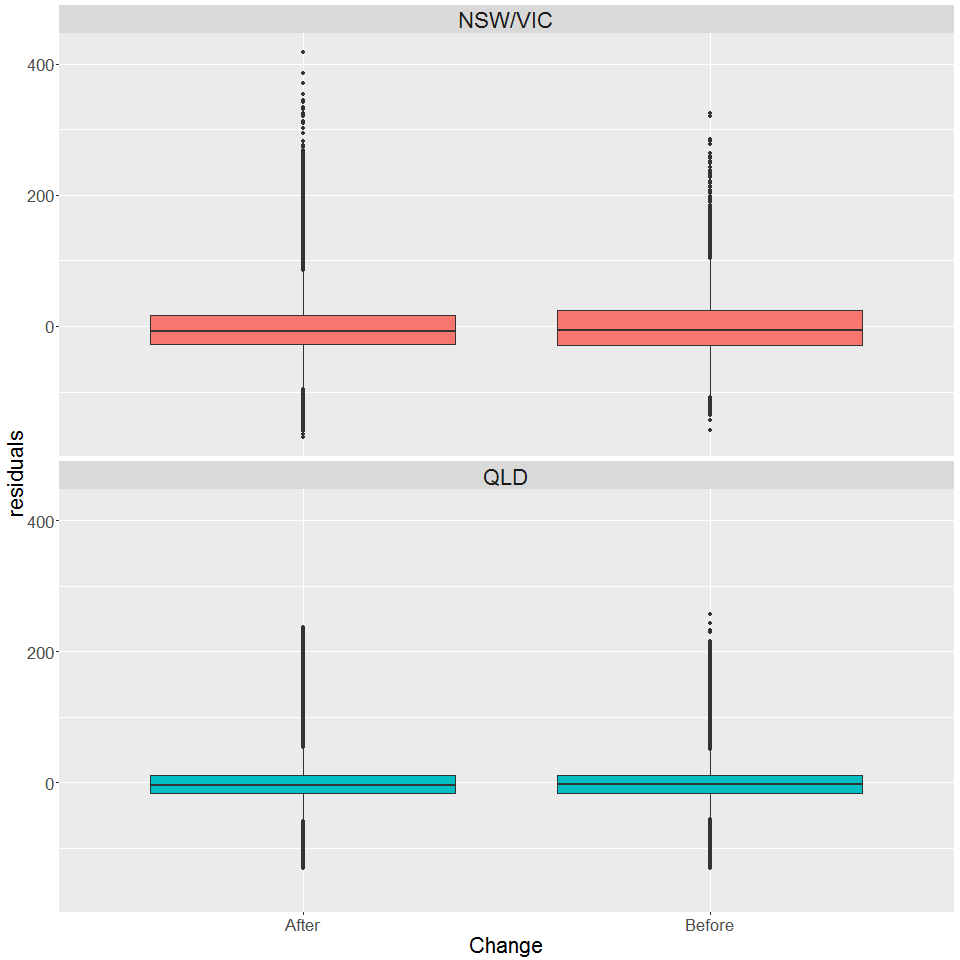
\includegraphics[width=0.7\linewidth]{figures/ResidualBoxplotchange} \caption{Boxplots of annual rainfall residuals (estimated based on Equation 2 before and after the land cover intervention during 1979 - 2015 in the study regions. On average, the after period has a significantly lower annual rainfall residual in NSW/VIC, but a signifcantly higher annual rainfall residual in the Qld study area}\label{fig:meandiff}
\end{figure}

The rainfall regression residuals without the landcover variable for the
two regions (before-change since 1979 and after-change) were also
compared (Figure \ref{fig:meandiff}) using a simple t-test. From the
boxplots it is difficult to see that there were significantly different
(\(p < 0.05\)) mean rainfall residual values between the ``before'' and
``after'' periods in both regions. For the Queensland locations, the
mean monthly rainfall residuals were slightly lower (\(p < 0.05\)) after
the change in landcover (\(~ 0.45 mm/month\)). For the NSW/VIC locations
there was larger decrease in the mean monthly rainfall residual
(\(p < 0.05\)) post change (\(~ 1.5 mm/month\)).

The choice of the number of pixels averaged in the step trend test
(\(ns\)) has some impact on the test results (Hirsch and Gilroy 1985).
The cases of \(ns = 1\) and \(ns = 9\) were also tested. The results for
\(ns = 1\) showed a lower number of significant pixels (at \(p< 0.10\))
compared to the \(ns = 4\) test. The results from the \(ns = 9\) test
was not different from the \(ns = 4\) test. We therefore decided to stay
with \(ns = 4\). The power of the test does not change much after
\(ns = 4\), as shown by Hirsch and Gilroy (1985).

As part of the analysis, the ``field significance'' of the Z' score test
was considered to improve the interpretion of the step change at
regional scales from multiple local tests (Wilks 2006; Westra,
Alexander, and Zwiers 2013). Here, the bootstrapping resampling method
from Westra, Alexander, and Zwiers (2013) was used to evaluate the field
significance. This means the spatial structure of the pixels was
maintained, but the order of the years and months was changed by random
resampling. For each resampling, the test statistic identifies the
percentage of the pixels with a significant positive or negative step
change for the step trend test. The test statistics on 1000 resampled
replicates were used to develop the distribution of these percentage
values, and the observed fraction of significant Z' scores (at
\(p < 0.1\)) is plotted on the distribution (Figure \ref{fig:fieldsig}).
The results support the earlier Z' score results. Only the percentage
significant positive Z' scores, indicating a decrease in rainfall for
the NSW/VIC region as a result in a decrease in tree cover, falls on the
tail of the field significance distribution, while all the others are
well within the distribution. This suggests that the percentage of
significant positive Z' scores in the NSW/VIC region is least likely due
to a unique series of rainfall years, but is most likely due to changes
in landcover. In other words, in the NSW/VIC region it is most likely
that the change in landcover (decrease in tree cover) caused a decrease
in the rainfall.

\begin{figure}
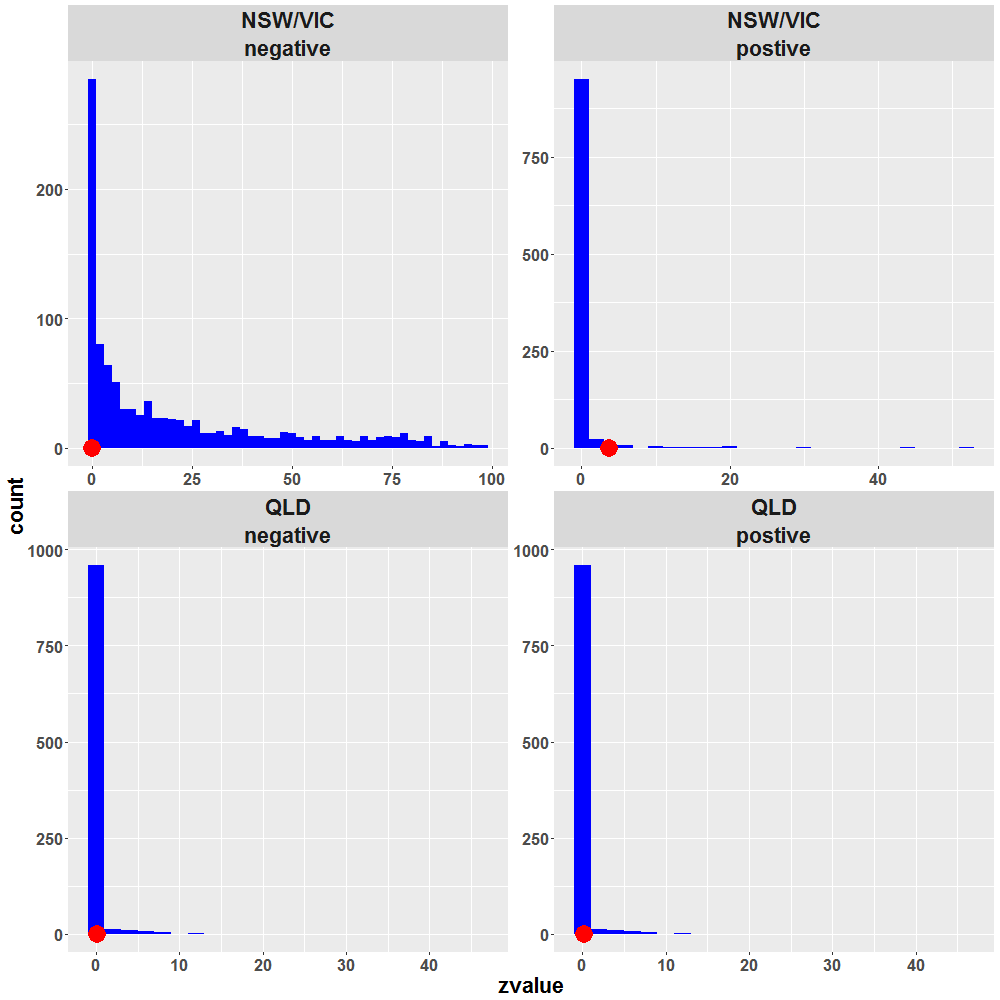
\includegraphics[width=0.7\linewidth]{figures/bt4_hist} \caption{Field significance results showing the distribution of percentage of significant Z' scores for the resampled series (blue bars), and the precentage significant Z' scores for the original series of rainfall years (red circle)}\label{fig:fieldsig}
\end{figure}

\section{Discussion}\label{discussion}

\begin{table}[t]

\caption{\label{tab:summarytable}Summary table of all tests on the two regions }
\centering
\resizebox{\linewidth}{!}{
\begin{tabular}{lll}
\toprule
Test & Qld & NSW VIC\\
\midrule
LC variable & Small area of significant pixels in the centre & Large area possibly aligning with bushfire affected area.\\
t-test regression model residuals & Slightly lower mean residual ($p<0.05$) after change (0.5 mm per month) & Lower mean residual ($p<0.05$) after change (1.5 mm per month)\\
Positive score & 0.2\% of pixels at $p<0.1$ & 3.7\% of pixel at $p<0.1$\\
Field significance \% of scores & Both positive and negative \% within random distribution & Positive \% outside random distribution.\\
\bottomrule
\end{tabular}}
\end{table}

Overall the summary table of the results indicates that the effects of
land clearing or bushfire on rainfall are consistent across the range of
different statistical tests. In all cases, the data for the NSW/VIC
region indicates the strongest evidence that the reduction in tree cover
(the land cover change) resulted in a local decrease in rainfall. In
contrast the data for the QLD region only indicates weak evidence that
the loss of trees due to land clearing resulted in reduction in the
rainfall.

Generally, empirical studies on LCC-precipitation interaction are
conducted within an area with known land surface intervention (e.g.
Otterman et al. 1990; Durieux, Machado, and Laurent 2003; Negri et al.
2004; Sato, Kimura, and Hasegawa 2007). However, these locations are
rare and difficult to isolate from real landscape change. Modelling
studies are abundant (e.g. Chagnon and Bras 2005; Pinto et al. 2009;
Wang et al. 2009), but these are generally not directly linked to
observed data. In this study we tested the effect of land cover change
across a broad region, which included locations where changes were known
to occur or have occured. The advantage of the current approach is that
long time series of land cover data are not required. This is
advantageous as this type of that is currently not always available.
Furthermore, it does not assume a specific relationship between
vegetation cover change and rainfall but allows the data to show this
relationship, by applying the analysis to a broader area outside the
boundary of the vegetation cover change. This approach is expected to
provide a way to reduce the risk of a false positive paradox, by
comparing results between areas with and without vegetation cover
change.

Overall the results suggest that at least for the NSW/VIC region that a
decrease in tree cover causes a decrease in rainfall (Figure
\ref{fig:tctrend}). However, there are several possible complicating
factors in the data that require discussion.

\subsection{Rainfall variability}\label{rainfall-variability}

Rainfall in Australia is highly variable from year to year, and the time
period in this study included a severe drought (Dijk and Viney 2013), as
well as the drought breaking years 2010 and 2011. The purpose of using
the regression model is to remove the year to year and month to month
variability in rainfall and therefore strengthen the land cover signal
in the residuals. We used the spatially averaged monthly rainfall
timeseries for the larger Murray Darling Basin (Figure \ref{fig:selreg})
to remove the general variability. However, overall the model does not
explain more than 50\% (QLD) and 30\% (NSW/VIC) of the rainfall
variability, and only around 7\% on average is due to the climate
drivers (Figure \ref{fig:rsq}) . And while this is consistent with the
literature e.g. Westra and Sharma (2010), this means some variation due
to external factors could still be left in the residuals. Rainfall is
generally considered a stochastic process (e.g. Fowler et al. 2005;
Cowpertwait, Salinger, and Mullen 2009; Burton et al. 2010) and some of
the variability could either be a different response to a combination of
climate factors (as interactions were not tested in the model), or a
non-stationary response to the climate drivers. The severe bushfires in
2003 were also triggered by the extreme drought conditions during the
millenium drought (Dijk and Viney 2013). Although the effect of the
drought on the overall rainfall quantities has been accounted for in
part by the model, a further delayed or cumulative effect of the drought
could be feeding into the local land-atmosphere interaction. As a
result, the rainfall feedback to the vegetation cover change could be
weak under the dry conditions between 2001 and 2009, and this could have
affected the result.

\subsection{Vegetation dynamics}\label{vegetation-dynamics}

The second possible effect is the dynamic nature of the vegetation
clearing and recovery, especially for the QLD region. Although land
clearing has occurred at a high rate and broad scale in Queensland
(Department of Science, Information Technology and Innovation 2017), the
clearing does not have a clear start and end point. QLD has a long
history of land clearing. According to the series of SLATS reports on
land cover changes in QLD released by the Queensland government, land
clearing continued in and around the study region between 1988 - 2008.
Major broad scale and high rate clearings occurred in 1999 - 2000 and
2002 - 2004 (Figure \ref{fig:slat}). And even though there was a
decrease in land clearing post 2005, it is difficult to define a clear
cut change in the tree cover in this region. The specific vegetation
class in the Queensland area is also well-known for rapid regrowth and
``thickening'' in favourable conditions (Gowen and Bray 2016), and this
could explain the increase in vegetation cover in 2015 in the Qld area
(Figure \ref{fig:tctrend}). In particular the favourable rainfall years
of 2010 and 2011 would have boosted regrowth, increasing
evapotranspiration and therefore decreasing the effect of the rainfall
change.

\begin{figure}
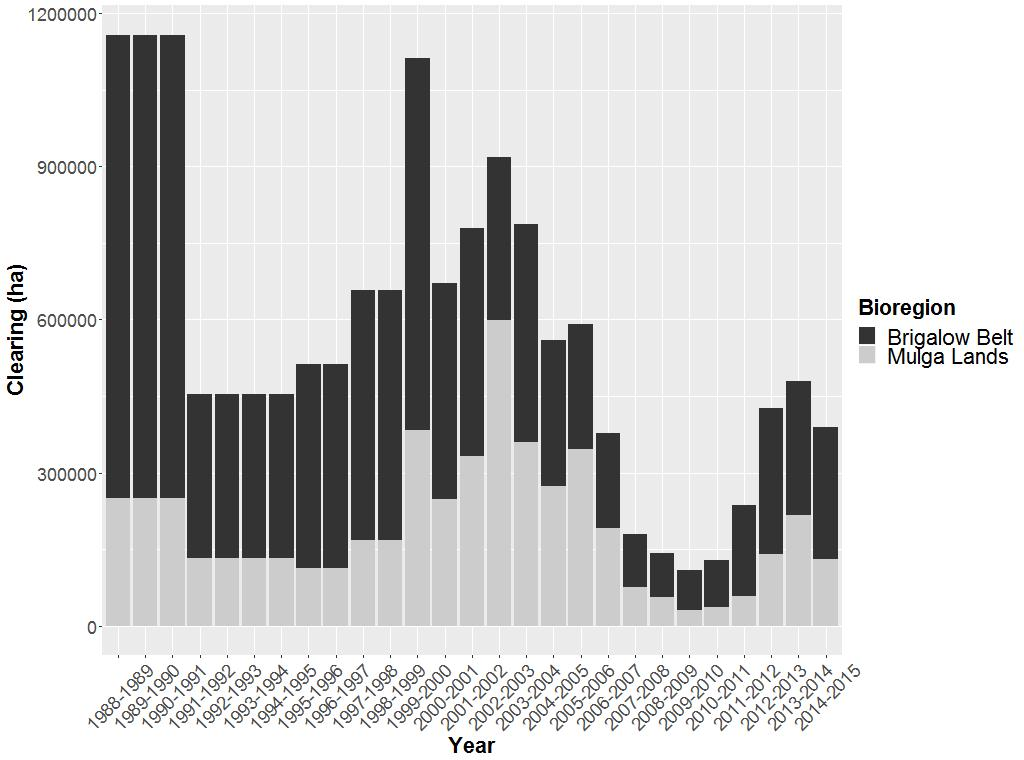
\includegraphics[width=0.9\linewidth]{figures/slats} \caption{Woody vegetation clearing rate in QLD for the two major bioregions in the study area. The data were obtained from SLATS (2017), and clearly indicate a sharp decrease in the clearing rate after 2005.}\label{fig:slat}
\end{figure}

The different causes of vegetation cover change in these two regions
could lead to different post-change characteristics. The trends in EVI
in the QLD region are opposite to the NSW/VIC region, based on the DLCD
data. This could also be due to the lower tree density in the QLD region
compared to the NSW/VIC region before land surface interventions. In
contrast, the significant bushfires (Figure \ref{fig:bushfire}) would
have drastically reduced the vegetation cover and recovery was very slow
in some areas within the NSW/VIC area. The persistent drought in the
2000s (Howden 2012; Dijk and Viney 2013) delayed the regrowth of trees.
Conversely, replacing tree cover with pasture and crops in the Qld area
might only have a relatively subtle impact on the EVI.

\subsection{Gridded monthly rainfall
data}\label{gridded-monthly-rainfall-data}

The rainfall data used in this study is gridded. This data set is robust
and consistent over a long time series (from 1900 to current) and has a
broad national wide coverage which can provide more information
spatially (Jeffrey et al. 2001; Tozer, Kiem, and Verdon-Kidd 2009).
However, high cross correlation between pixels, due to the interpolation
method in this data set (Jeffrey et al. 2001), can also introduce
spatial noise. In the step trend test the cross correlation was
accounted for. However, some other methods are also available, which
could be used to perform a comparative trial. For example, Narisma et
al. (2007) applied a spatial Gaussian filter on a similar data set and
used wavelet analysis to detect a step change in rainfall. High quality
station data is another option to test whether the observed spatial
pattern in the step trend test results was not due to the gridded data
itself. Resampling methods, such as bootstrapping and permutation (used
in this study) (Wilks 1997; Kundzewicz and Robson 2004; Westra,
Alexander, and Zwiers 2013), can also be used to further assess the
strength of the significance of results . While the gridded data set is
most useful in regions with sparse rain gauge networks, such as in this
study, it can actually reduce information where the rain gauge density
is high (Jones, Wang, and Fawcett 2009). In the NSW/VIC region, the
coverage of rainfall stations is more intensive, but they are mainly
located in the valleys. As a result, the interpolated data might be a
limited representation of the true local rainfall.

\subsection{General approach}\label{general-approach}

Parametric tests are generally more powerful than nonparametric test in
detecting a trend, when the data is normally distributed (Onoz and
Bayazit 2003; Kundzewicz and Robson 2004). As a non-parametric test, the
step trend test has the advantage of being distribution free and having
no restriction on missing data (Hirsch and Gilroy 1985). This is
particularly useful in rainfall analysis since rainfall data is usually
highly skewed. On the other hand, the disadvantages of non-parametric
tests, such as being limited to hypothesis testing and being weaker in
power, also hold for the step trend test (Whitley and Ball 2002).

Overall, the current study provides a statistical data based approach,
building on several lines of evidence to reject the null hypothesis (no
step change in rainfall occurs as a result of tree cover loss) at least
for the NSW/VIC region. Limited by the available data, the time frame
under study included a long lasting drought period (Holper 2011; Dijk
and Viney 2013). The strong impact of this prolonged drought might have
suppressed the land-atmosphere interaction and modified the cause and
effect relationship between rainfall and vegetation cover change. This
could be one of the reasons that the land cover change effects on the
local climate found in other studies (e.g. Görgen et al. 2006; McAlpine
et al. 2007) do not appear in the QLD region. Possible future work could
focus on a non-drought period, or using a different series of land cover
data, possibly on another continent. The recent large bushfires on the
US continent come to mind as a possible candidate study once sufficient
post event data is collected. Wile the power of the test can be improved
with the longer length of the post-intervention period (Hirsch and
Gilroy 1985), the dynamic nature of vegetation regrowth in this case
study also affects this effect. A better approach might be to build a
global study that investigates multiple locations where drastic
landcover changes have taken place, which would also remove some of the
climate variability effects due to the larger sample size.

\section{Conclusions}\label{conclusions}

In this study, we present a statistical approach to identify the impact
of a change in land cover on local rainfall.The results, based on
gridded rainfall data found, that a reduction in vegetation cover is
likely to have reduced local rainfall for a large area in NSW/VIC
affected by bushfires. However, land clearing in QLD was unlikely to
have reduced rainfall over the same time period.

Drought may have had a pronounced impact on the land surface condition
during the study period, also leading to significant reduction in
vegetation cover and extreme events such as bushfires. The lack of
rainfall and associated high temperatures may mask the impact on
rainfall of a step change in the vegetation cover. Hence, the signal of
Land Cover Change feedback on rainfall is probably weaker under such
regional dry conditions, as the impact of Land Cover Change on rainfall
is mainly through changes in moisture convergence (Görgen et al. 2006;
Pitman and Hesse 2007).

\section{appendix}\label{appendix}

\emph{Summary of Data}

\begin{sidewaystable}
 \caption{Summary of data.}
  \label{tab:ch3Data}
 \begin{tabular}{lllll}
  \hline
  \textbf{Data} & \textbf{Source} & \multicolumn{2}{c}{\textbf{Resolution}} & \textbf{Analysis period} \\\cline{3-4}
  & & Temporal & Spatial & \\\hline
  Percent tree cover & MOD44B & Annual &    250m & 2000-2010\\
  Trend of vegetation cover change  &   DLCD (2009) & Onetime & 250m    & Trend of Apr 2000 - Apr 2008\\
  Rainfall &    AWAP gridded rainfall data &    Monthly &   0.05\textdegree$\times$0.05\textdegree & Jan 1979- Dec 2008\\
  SOI   & BoM   & Monthly & N/A &   Jan 1979- Dec 2008\\
  NINO 3, 3.4, 4 &  IRI/LDEO data library   & Monthly   & N/A   & Jan 1979- Dec 2008\\
  PDO   & NOAA & Monthly    & N/A   & Jan 1979- Dec 2008\\
  IOD   & POAMA-2 dataset   & Monthly   & N/A   & Jan 1979- Dec 2008\\
  \hline
  \end{tabular}
\end{sidewaystable}

\newpage

\section*{References}\label{references}
\addcontentsline{toc}{section}{References}

\hypertarget{refs}{}
\hypertarget{ref-ABARES2010}{}
ABARES. 2010. ``Land Use of Australia, Version 4, 2005/2006.''

\hypertarget{ref-ABC2003}{}
ABC News. 2003. ``Kosciuszko Slow to Recover from Bushfires.''

\hypertarget{ref-ABS2012}{}
Australian Bureau of Statistics. 2012. ``Geography and Climate -
Australia's Climate.''

\hypertarget{ref-Ben-Gai1998}{}
Ben-Gai, T., A. Bitan, A. Manes, P. Alpert, and S. Rubin. 1998.
``Spatial and Temporal Changes in Rainfall Frequency Distribution
Patterns in Israel.'' \emph{Theoretical and Applied Climatology} 61
(3-4): 177--90.
\href{\%3CGo\%20to\%20ISI\%3E://000078025000005}{\textless{}Go to ISI\textgreater{}://000078025000005}.

\hypertarget{ref-BoM2012a}{}
BoM. 2012a. ``Australia - Climate of Our Continent.''

\hypertarget{ref-BoM2012}{}
---------. 2012b. ``Australian Climate Influence.''

\hypertarget{ref-Bosilovich2006}{}
Bosilovich, Michael G., and Jiun-Dar Chern. 2006. ``Simulation of Water
Sources and Precipitation Recycling for the MacKenzie, Mississippi, and
Amazon River Basins.'' \emph{Journal of Hydrometeorology} 7 (3):
312--29. \url{http://dx.doi.org/10.1175\%2FJHM501.1}.

\hypertarget{ref-Burton2010}{}
Burton, A, HJ Fowler, S Blenkinsop, and CG Kilsby. 2010. ``Downscaling
Transient Climate Change Using a Neyman-Scott Rectangular Pulses
Stochastic Rainfall Model.'' \emph{Journal of Hydrology} 381 (1):
18--32.

\hypertarget{ref-Chagnon2005}{}
Chagnon, F. J. F., and R. L. Bras. 2005. ``Contemporary Climate Change
in the Amazon.'' \emph{Geophysical Research Letters} 32 (13).

\hypertarget{ref-Chowdhury2010}{}
Chowdhury, R. K., and S. Beecham. 2010. ``Australian Rainfall Trends and
Their Relation to the Southern Oscillation Index.'' \emph{Hydrological
Processes} 24 (4). John Wiley \& Sons, Ltd.: 504--14.
\url{http://dx.doi.org/10.1002/hyp.7504}.

\hypertarget{ref-Cowpertwait2009}{}
Cowpertwait, PSP, Jim Salinger, and B Mullen. 2009. ``A Spatial-Temporal
Stochastic Rainfall Model for Auckland City: Scenarios for Current and
Future Climates.'' \emph{Journal of Hydrology (NZ)} 48: 95--109.

\hypertarget{ref-Deo2009}{}
Deo, RC, JI Syktus, CA McAlpine, and KK Wong. 2009. ``The Simulated
Impact of Land Cover Change on Climate Extremes in Eastern Australia.''
In \emph{Proceedings of the 18th World Imacs Congress and Modsim09
International Congress on Modelling and Simulation}, 2035--41.
Modelling; Simulation Society of Australia; New Zealand Inc.;
International Association for Mathematics; Computers in Simulation.

\hypertarget{ref-SLATS2001}{}
Department of Natural Resources and Mines. 2005. ``Land Cover Change in
Queensland 2001-2003, Incorporating 2001-2002 Adn 2002-2003 Change
Periods: A Statewide Landcover and Trees Study (SLATS) Report.''
Brisbane: Department of Natural Resources; Mines.

\hypertarget{ref-SLATS2004}{}
Department of Natural Resources and Water. 2007. ``Land Cover Change in
Queensland 2004-2005: A Statewide Landcover and Trees Study (SLATS)
Report.'' Brisbane: Department of Natural Resources; Water.

\hypertarget{ref-SLATS2017}{}
Department of Science, Information Technology and Innovation. 2017.
``Land Cover Change in Queensland 2015-2016: A Statewide Landcover and
Trees Study (SLATS) Report.'' Brisbane: Department of Science,
Information Technology; Innovation.

\hypertarget{ref-vanDijk2013}{}
Dijk, Beck van, Albert I. J. M., and Neil R. Viney. 2013. ``The
Millennium Drought in Southeast Australia (2001--2009): Natural and
Human Causes and Implications for Water Resources, Ecosystems, Economy,
and Society.'' \emph{Water Resources Research} 49 (2): 1040--57.
doi:\href{https://doi.org/10.1002/wrcr.20123}{10.1002/wrcr.20123}.

\hypertarget{ref-Dirmeyer2009}{}
Dirmeyer, P. A., K. L. Brubaker, and T. DelSole. 2009. ``Import and
Export of Atmospheric Water Vapor Between Nations.'' \emph{Journal of
Hydrology} 365 (1-2): 11--22.
\href{\%3CGo\%20to\%20ISI\%3E://000263575600003}{\textless{}Go to ISI\textgreater{}://000263575600003}.

\hypertarget{ref-Durieux2003}{}
Durieux, Laurent, Luiz Augusto Toledo Machado, and Henri Laurent. 2003.
``The Impact of Deforestation on Cloud Cover over the Amazon Arc of
Deforestation.'' \emph{Remote Sensing of Environment} 86 (1): 132--40.

\hypertarget{ref-Eltahir1996}{}
Eltahir, E. A. B., and R. L. Bras. 1996. ``Precipitation Recycling.''
\emph{Reviews of Geophysics} 34 (3): 367--78.
\href{\%3CGo\%20to\%20ISI\%3E://A1996VD58700003}{\textless{}Go to ISI\textgreater{}://A1996VD58700003}.

\hypertarget{ref-Fowler2005}{}
Fowler, HJ, CG Kilsby, PE O'connell, and A Burton. 2005. ``A
Weather-Type Conditioned Multi-Site Stochastic Rainfall Model for the
Generation of Scenarios of Climatic Variability and Change.''
\emph{Journal of Hydrology} 308 (1): 50--66.

\hypertarget{ref-Gaertner2001}{}
Gaertner, M. A., O. B. Christensen, J. A. Prego, J. Polcher, C.
Gallardo, and M. Castro. 2001. ``The Impact of Deforestation on the
Hydrological Cycle in the Western Mediterranean: An Ensemble Study with
Two Regional Climate Models.'' \emph{Climate Dynamics} 17 (11): 857--73.

\hypertarget{ref-Gallant2007}{}
Gallant, Ailie J. E., Kevin J. Hennessy, and James Risbey. 2007.
``Trends in Rainfall Indices for Six Australian Regions: 1910 - 2005.''
\emph{Australian Meteorological Magazine} 56: 223--39.

\hypertarget{ref-Gimeno2010}{}
Gimeno, Luis, Anita Drumond, Raquel Nieto, Ricardo M. Trigo, and Andreas
Stohl. 2010. ``On the Origin of Continental Precipitation.''
\emph{Geophysical Research Letters} 37 (13). AGU.
\url{http://dx.doi.org/10.1029/2010GL043712}.

\hypertarget{ref-Gowen2016}{}
Gowen, Rebecca, and Steven G. Bray. 2016. ``Bioeconomic Modelling of
Woody Regrowth Carbon Offset Options in Productive Grazing Systems.''
\emph{The Rangeland Journal} 38 (3): 307--17.
doi:\href{https://doi.org/https://doi.org/10.1071/RJ15084}{https://doi.org/10.1071/RJ15084}.

\hypertarget{ref-Gorgen2006}{}
Görgen, K., A. H. Lynch, A. G. Marshall, and J. Beringer. 2006. ``Impact
of Abrupt Land Cover Changes by Savanna Fire on Northern Australian
Climate.'' \emph{Journal of Geophysical Research-Atmospheres} 111 (D19):
D19106. \url{http://dx.doi.org/10.1029/2005JD006860}.

\hypertarget{ref-Hastie1986}{}
Hastie, Trevor, and Robert Tibshirani. 1986. ``Generalized Additive
Models.'' \emph{Statistical Science}, 297--310.

\hypertarget{ref-Hipel1994}{}
Hipel, K.W., and A.I. McLeod. 1994. \emph{Time Series Modelling of Water
Resources and Environmental Systems}. Vol. 45. Elsevier Science Ltd.

\hypertarget{ref-Hirsch1985}{}
Hirsch, Robert M., and Edward J. Gilroy. 1985. ``Detectability of Step
Trends in the Rate of Atmospheric Deposition of Sulfate.'' \emph{JAWRA
Journal of the American Water Resources Association} 21 (5): 773--84.
\url{http://dx.doi.org/10.1111/j.1752-1688.1985.tb00171.x}.

\hypertarget{ref-Holper2011}{}
Holper, Paul N. 2011. \emph{Climate Change, Science Information Paper:
Australian Rainfall-Past, Present and Future}. Canberra: CSIRO.

\hypertarget{ref-Howden2012}{}
Howden, Saffron. 2012. ``It's Official: Australia No Longer in
Drought.'' \emph{Brisbane Times}.

\hypertarget{ref-Hughes2003}{}
Hughes, Lesley. 2003. ``Climate Change and Australia: Trends,
Projections and Impacts.'' \emph{Austral Ecology} 28 (4). Blackwell
Science Pty: 423--43.
\url{http://dx.doi.org/10.1046/j.1442-9993.2003.01300.x}.

\hypertarget{ref-SILO2001}{}
Jeffrey, Stephen J., John O. Carter, Keith B. Moodie, and Alan R.
Beswick. 2001. ``Using Spatial Interpolation to Construct a
Comprehensive Archive of Australian Climate Data.'' Journal Article.
\emph{Environmental Modelling \& Software} 16 (4 SU -): 309--30.
\url{http://www.sciencedirect.com/science/article/B6VHC-42SXF8F-2/2/b5c0a24b85149f40ba5d2419ddc0999c}.

\hypertarget{ref-Jones2009}{}
Jones, D.A., W. Wang, and R. Fawcett. 2009. ``High-Quality Spatial
Climate Data-Sets for Australia.'' \emph{Australian Meteorological and
Oceanographic Journal} 58 (4): 233--48.

\hypertarget{ref-Junkermann2009}{}
Junkermann, W., J. Hacker, T. Lyons, and U. Nair. 2009. ``Land Use
Change Suppresses Precipitation.'' \emph{Atmospheric Chemistry and
Physics} 9 (17): 6531--9.
\href{\%3CGo\%20to\%20ISI\%3E://WOS:000269778500018}{\textless{}Go to ISI\textgreater{}://WOS:000269778500018}.

\hypertarget{ref-Kamruzzaman2011}{}
Kamruzzaman, M., S. Beecham, and A. V. Metcalfe. 2011.
``Non-Stationarity in Rainfall and Temperature in the Murray Darling
Basin.'' \emph{Hydrological Processes} 25 (10). John Wiley \& Sons,
Ltd.: 1659--75. \url{http://dx.doi.org/10.1002/hyp.7928}.

\hypertarget{ref-Koutsoyiannis2007}{}
Koutsoyiannis, Demetris. 2006. ``Nonstationarity Versus Scaling in
Hydrology.'' Journal Article. \emph{Journal of Hydrology} 324 (1-4):
239--54.
\href{http://www.sciencedirect.com/science/article/B6V6C-4HP6GJ9-1/2/67dcc2e8f8e75b7abb918617f5a79a37\%20}{http://www.sciencedirect.com/science/article/B6V6C-4HP6GJ9-1/2/67dcc2e8f8e75b7abb918617f5a79a37}.

\hypertarget{ref-kucharski_further_2013}{}
Kucharski, Fred, Ning Zeng, and Eugenia Kalnay. 2013. ``A Further
Assessment of Vegetation Feedback on Decadal Sahel Rainfall
Variability.'' \emph{Climate Dynamics} 40 (5-6): 1453--66.
\url{http://link.springer.com/article/10.1007/s00382-012-1397-x}.

\hypertarget{ref-Kuzcera1987}{}
Kuczera, George. 1987. ``Prediction of Water Yield Reductions Following
a Bushfire in Ash-Mixed Species Eucalypt Forest.'' \emph{Journal of
Hydrology} 94 (3-4): 215--36.
doi:\href{https://doi.org/https://10.1016/0022-1694(87)90054-0}{https://10.1016/0022-1694(87)90054-0}.

\hypertarget{ref-Kundzewicz2004}{}
Kundzewicz, Z.W., and A.J. Robson. 2004. ``Change Detection in
Hydrological Records-a Review of the Methodology/Revue Méthodologique de
La Détection de Changements Dans Les Chroniques Hydrologiques.''
\emph{Hydrological Sciences Journal} 49 (1).

\hypertarget{ref-Lymburner2010}{}
Lymburner, Leo, Peter Tan, Norman Mueller, Richard Thackway, Adam Lewis,
Medhavy Thankappan, Lucy Randall, Anisul Islam, and Udaya Senarath.
2010. ``250 Metre Dynamic Land Cover Dataset.'' Geoscience Australia,
Canberra.

\hypertarget{ref-Ma2011}{}
Ma, H. Y., C. R. Mechoso, Y. Xue, H. Xiao, C. M. Wu, J. L. Li, and F. De
Sales. 2011. ``Impact of Land Surface Processes on the South American
Warm Season Climate.'' \emph{Climate Dynamics} 37 (1-2): 187--203.
\href{\%3CGo\%20to\%20ISI\%3E://WOS:000293403000012}{\textless{}Go to ISI\textgreater{}://WOS:000293403000012}.

\hypertarget{ref-MacDonald2005}{}
MacDonald, Glen M., and Roslyn A. Case. 2005. ``Variations in the
Pacific Decadal Oscillation over the Past Millennium.''
\emph{Geophysical Research Letters} 32 (8): L08703.
\url{http://dx.doi.org/10.1029/2005GL022478}.

\hypertarget{ref-McAlpine2007}{}
McAlpine, C. A., J. Syktus, R. C. Deo, P. J. Lawrence, H. A. McGowan, I.
G. Watterson, and S. R. Phinn. 2007. ``Modeling the Impact of Historical
Land Cover Change on Australia's Regional Climate.'' \emph{Geophysical
Research Letters} 34 (22).
\href{\%3CGo\%20to\%20ISI\%3E://000251345100005}{\textless{}Go to ISI\textgreater{}://000251345100005}.

\hypertarget{ref-Mei2010}{}
Mei, R., and G. L. Wang. 2010. ``Rain Follows Logging in the Amazon?
Results from CAM3-CLM3.'' \emph{Climate Dynamics} 34 (7-8): 983--96.
\href{\%3CGo\%20to\%20ISI\%3E://WOS:000278088400005}{\textless{}Go to ISI\textgreater{}://WOS:000278088400005}.

\hypertarget{ref-Meneghini2007}{}
Meneghini, Belinda, Ian Simmonds, and Ian N. Smith. 2007. ``Association
Between Australian Rainfall and the Southern Annular Mode.''
\emph{International Journal of Climatology} 27 (1): 109--21.
\url{http://dx.doi.org/10.1002/joc.1370}.

\hypertarget{ref-Murphy2008}{}
Murphy, Bradley F., and Bertrand Timbal. 2008. ``A Review of Recent
Climate Variability and Climate Change in Southeastern Australia.''
\emph{International Journal of Climatology} 28 (7): 859--79.
\url{http://dx.doi.org/10.1002/joc.1627}.

\hypertarget{ref-Nair2011}{}
Nair, Udaysankar S., Y. Wu, J. Kala, T. J. Lyons, Sr. Pielke R. A., and
J. M. Hacker. 2011. ``The Role of Land Use Change on the Development and
Evolution of the West Coast Trough, Convective Clouds, and Precipitation
in Southwest Australia.'' \emph{Journal of Geophysical
Research-Atmospheres} 116 (D7). AGU: D07103.
\url{http://dx.doi.org/10.1029/2010JD014950}.

\hypertarget{ref-Narisma2007}{}
Narisma, G.T., J.A. Foley, R. Licker, and N. Ramankutty. 2007. ``Abrupt
Changes in Rainfall During the Twentieth Century.'' \emph{Geophysical
Research Letters} 34 (6): L06710.

\hypertarget{ref-Negri2004}{}
Negri, A. J., R. F. Adler, L. M. Xu, and J. Surratt. 2004. ``The Impact
of Amazonian Deforestation on Dry Season Rainfall.'' \emph{Journal of
Climate} 17 (6): 1306--19.

\hypertarget{ref-Nicholls2006}{}
Nicholls, N. 2006. ``Detecting and Attributing Australian Climate
Change: A Review.'' \emph{Australian Meteorological Magazine} 55 (3).
Bureau of Meteorology.: 199--211.

\hypertarget{ref-Oleson2004}{}
Oleson, K. W., G. B. Bonan, S. Levis, and M. Vertenstein. 2004.
``Effects of Land Use Change on North American Climate: Impact of
Surface Datasets and Model Biogeophysics.'' \emph{Climate Dynamics} 23
(2): 117--32.

\hypertarget{ref-Onoz2003}{}
Onoz, B., and M. Bayazit. 2003. ``The Power of Statistical Tests for
Trend Detection.'' \emph{Turkish Journal of Engineering and
Environmental Sciences} 27 (4): 247--51.

\hypertarget{ref-Otterman1990}{}
Otterman, J., A. Manes, S. Rubin, P. Alpert, and D. Starr. 1990. ``An
Increase of Early Rains in Southern Israel Following Land-Use Change?''
\emph{Boundary-Layer Meteorology} 53 (4): 333--51.

\hypertarget{ref-Pinto2009}{}
Pinto, E., Y. Shin, S. A. Cowling, and C. D. Jones. 2009. ``Past,
Present and Future Vegetation-Cloud Feedbacks in the Amazon Basin.''
\emph{Climate Dynamics} 32 (6): 741--51.
\href{\%3CGo\%20to\%20ISI\%3E://WOS:000264118400001}{\textless{}Go to ISI\textgreater{}://WOS:000264118400001}.

\hypertarget{ref-Pitman2007}{}
Pitman, A. J., and P. P. Hesse. 2007. ``The Significance of Large-Scale
Land Cover Change on the Australian Palaeomonsoon.'' \emph{Quaternary
Science Reviews} 26 (1-2): 189--200.

\hypertarget{ref-pitman_scale_2016}{}
Pitman, A. J., and R. Lorenz. 2016. ``Scale Dependence of the Simulated
Impact of Amazonian Deforestation on Regional Climate.''
\emph{Environmental Research Letters} 11 (9): 094025.
doi:\href{https://doi.org/10.1088/1748-9326/11/9/094025}{10.1088/1748-9326/11/9/094025}.

\hypertarget{ref-Pitman2004}{}
Pitman, A. J., G. T. Narisma, R. A. Pielke, and N. J. Holbrook. 2004.
``Impact of Land Cover Change on the Climate of Southwest Western
Australia.'' \emph{Journal of Geophysical Research-Atmospheres} 109
(D18).
\href{\%3CGo\%20to\%20ISI\%3E://WOS:000224126500001}{\textless{}Go to ISI\textgreater{}://WOS:000224126500001}.

\hypertarget{ref-Rstats2018}{}
R Core Team, 2018. \emph{R: A Language and Environment for Statistical
Computing}. Vienna, Austria: R Foundation for Statistical Computing.
\url{http://www.R-project.org/}.

\hypertarget{ref-Risbey2009}{}
Risbey, James S., Michael J. Pook, Peter C. McIntosh, Matthew C.
Wheeler, and Harry H. Hendon. 2009. ``On the Remote Drivers of Rainfall
Variability in Australia.'' \emph{Monthly Weather Review} 137 (10):
3233--53. \url{http://dx.doi.org/10.1175/2009MWR2861.1}.

\hypertarget{ref-Roy2008}{}
Roy, David P, Luigi Boschetti, Christopher O Justice, and J Ju. 2008.
``The Collection 5 Modis Burned Area Product---Global Evaluation by
Comparison with the Modis Active Fire Product.'' \emph{Remote Sensing of
Environment} 112 (9). Elsevier: 3690--3707.

\hypertarget{ref-Roy2005}{}
Roy, DP, Y Jin, PE Lewis, and CO Justice. 2005. ``Prototyping a Global
Algorithm for Systematic Fire-Affected Area Mapping Using Modis Time
Series Data.'' \emph{Remote Sensing of Environment} 97 (2). Elsevier:
137--62.

\hypertarget{ref-Roy2002}{}
Roy, DP, PE Lewis, and CO Justice. 2002. ``Burned Area Mapping Using
Multi-Temporal Moderate Spatial Resolution Data---A Bi-Directional
Reflectance Model-Based Expectation Approach.'' \emph{Remote Sensing of
Environment} 83 (1). Elsevier: 263--86.

\hypertarget{ref-saha_investigating_2016}{}
Saha, Subodh K., Paul A. Dirmeyer, and Thomas N. Chase. 2016.
``Investigating the Impact of Land-Use Land-Cover Change on Indian
Summer Monsoon Daily Rainfall and Temperature During 1951-2005 Using a
Regional Climate Model.'' \emph{Hydrology and Earth System Sciences} 20
(5): 1765.
\url{http://search.proquest.com/openview/c4242c9ecce075e3545390b1d00f2751/1?pq-origsite=gscholar\&cbl=105724}.

\hypertarget{ref-Saji1999}{}
Saji, NH, B.N. Goswami, PN Vinayachandran, and T. Yamagata. 1999. ``A
Dipole Mode in the Tropical Indian Ocean.'' \emph{Nature} 401 (6751):
360--63.

\hypertarget{ref-Sato2007}{}
Sato, T., F. Kimura, and A. S. Hasegawa. 2007. ``Vegetation and
Topographic Control of Cloud Activity over Arid/Semiarid Asia.''
\emph{Journal of Geophysical Research-Atmospheres} 112 (D24).

\hypertarget{ref-Schepen2012}{}
Schepen, Andrew, Q. J. Wang, and David Robertson. 2012. ``Evidence for
Using Lagged Climate Indices to Forecast Australian Seasonal Rainfall.''
\emph{Journal of Climate} 25 (4). American Meteorological Society:
1230--46.

\hypertarget{ref-Semazzi2001}{}
Semazzi, F. H. M., and Y. Song. 2001. ``A GCM Study of Climate Change
Induced by Deforestation in Africa.'' \emph{Climate Research} 17 (2):
169--82.

\hypertarget{ref-Smith2012}{}
Smith, Ian N., and Bertrand Timbal. 2012. ``Links Between Tropical
Indices and Southern Australian Rainfall.'' \emph{International Journal
of Climatology} 32 (1): 33--40.

\hypertarget{ref-Speer2011}{}
Speer, Milton, Lance Leslie, and Alexandre Fierro. 2011. ``Australian
East Coast Rainfall Decline Related to Large Scale Climate Drivers.''
\emph{Climate Dynamics} 36 (7): 1419--29.
\url{http://dx.doi.org/10.1007/s00382-009-0726-1}.

\hypertarget{ref-Fire2011}{}
The State Government of Victoria. 2011. ``Bushfire History.''

\hypertarget{ref-Timbal2006}{}
Timbal, B., and J.M. Arblaster. 2006. ``Land Cover Change as an
Additional Forcing to Explain the Rainfall Decline in the South West of
Australia.'' \emph{Geophysical Research Letters} 33 (7): L07717.

\hypertarget{ref-Townshend2011}{}
Townshend, J.R.G., M. Carroll, C. Dimiceli, R. Sohlberg, M. Hansen, and
R. DeFries. 2011. ``Vegetation Continuous Fields MOD44B, 2001 Percent
Tree Cover, Collection 5.'' University of Maryland, College Park,
Maryland, 2001.

\hypertarget{ref-Beesley2009}{}
Tozer, C. R., A. S. Kiem, and D. C. Verdon-Kidd. 2009. ``On the
Uncertainties Associated with Using Gridded Rainfall Data as a Proxy for
Observed.'' Conference Paper. In \emph{18th World Imacs Congress and
Modsim09 International Congress on Modelling and Simulation.}, edited by
R.S. Anderssen, R.D. Braddock, and L.T.H. Newham, 3886--92.
\href{http://www.mssanz.org.au/modsim09/I13/beesley.pdf\%20}{http://www.mssanz.org.au/modsim09/I13/beesley.pdf}.

\hypertarget{ref-Tozer2012}{}
---------. 2012. ``On the Uncertainties Associated with Using Gridded
Rainfall Data as a Proxy for Observed.'' Journal Article. \emph{Hydrol.
Earth Syst. Sci.} 16 (5): 1481--99.
doi:\href{https://doi.org/10.5194/hess-16-1481-2012}{10.5194/hess-16-1481-2012}.

\hypertarget{ref-Trenberth1999}{}
Trenberth, K. E. 1999. ``Atmospheric Moisture Recycling: Role of
Advection and Local Evaporation.'' \emph{Journal of Climate} 12 (5):
1368--81.
\href{\%3CGo\%20to\%20ISI\%3E://000080145700002}{\textless{}Go to ISI\textgreater{}://000080145700002}.

\hypertarget{ref-Verdon2004}{}
Verdon, Danielle C., Adam M. Wyatt, Anthony S. Kiem, and Stewart W.
Franks. 2004. ``Multidecadal Variability of Rainfall and Streamflow:
Eastern Australia.'' \emph{Water Resources Research} 40 (10): W10201.
\url{http://dx.doi.org/10.1029/2004WR003234}.

\hypertarget{ref-Wang2009}{}
Wang, Jingfeng, Frederic Chagnon, Earle Williams, Alan Betts, Nilton
Renno, Luiz Machado, Gautam Bisht, Ryan Knox, and Rafael Bras. 2009.
``Impact of Deforestation in the Amazon Basin on Cloud Climatology.''
\emph{Proceedings of the National Academy of Sciences of the United
States of America} 106 (10): 3670.

\hypertarget{ref-Westra2013}{}
Westra, Seth, Lisa V. Alexander, and Francis W. Zwiers. 2013. ``Global
Increasing Trends in Annual Maximum Daily Precipitation.'' \emph{Journal
of Climate} 26 (11). American Meteorological Society: 3904--18.
\url{http://dx.doi.org/10.1175/JCLI-D-12-00502.1}.

\hypertarget{ref-Westra2010}{}
Westra, Seth, and Ashish Sharma. 2010. ``An Upper Limit to Seasonal
Rainfall Predictability?'' \emph{Journal of Climate} 23 (12). American
Meteorological Society: 3332--51.

\hypertarget{ref-Whitley2002}{}
Whitley, Elise, and Jonathan Ball. 2002. ``Statistics Review 6:
Nonparametric Methods.'' \emph{Critical Care, London} 6 (6): 509--13.

\hypertarget{ref-Wilks2006}{}
Wilks, D. S. 2006. ``On `Field Significance' and the False Discovery
Rate.'' \emph{Journal of Applied Meteorology and Climatology} 45 (9).
American Meteorological Society: 1181--9.

\hypertarget{ref-Wilks1997}{}
Wilks, DS. 1997. ``Resampling Hypothesis Tests for Autocorrelated
Fields.'' \emph{Journal of Climate} 10 (1): 65--82.

\hypertarget{ref-Wood2011}{}
Wood, S. N. 2011. ``Fast Stable Restricted Maximum Likelihood and
Marginal Likelihood Estimation of Semiparametric Generalized Linear
Models.'' \emph{Journal of the Royal Statistical Society (B)} 73 (1):
3--36.

\hypertarget{ref-Zanchettin2008}{}
Zanchettin, Davide, Stewart W. Franks, Pietro Traverso, and Mario
Tomasino. 2008. ``On Enso Impacts on European Wintertime Rainfalls and
Their Modulation by the Nao and the Pacific Multi-Decadal Variability
Described Through the Pdo Index.'' \emph{International Journal of
Climatology} 28 (8). John Wiley \& Sons, Ltd.: 995--1006.
\url{http://dx.doi.org/10.1002/joc.1601}.

\hypertarget{ref-Zeng2012}{}
Zeng, X. M., Z. H. Wu, S. Song, S. Y. Xiong, Y. Q. Zheng, Z. G. Zhou,
and H. Q. Liu. 2012. ``Effects of Land Surface Schemes on the Simulation
of a Heavy Rainfall Event by WRF.'' \emph{Chinese Journal of
Geophysics-Chinese Edition} 55 (1): 16--28.
\href{\%3CGo\%20to\%20ISI\%3E://WOS:000300129300002}{\textless{}Go to ISI\textgreater{}://WOS:000300129300002}.



\end{document}
